% !TeX program = xelatex
% Compilation : xelatex main.tex (2 passes pour le sommaire/numérotation)
% Nécessite XeLaTeX ou LuaLaTeX (fontspec) — pdflatex ne fonctionnera pas.
% Via Docker/Taskfile : task report (voir CLAUDE.md, Étape 5).
%
% Polices requises (à placer dans report/fonts/ si non installées système,
% téléchargeables gratuitement sur fonts.google.com — licence Apache) :
%   fonts/Poppins-Bold.ttf, Poppins-SemiBold.ttf, Poppins-Regular.ttf
%   fonts/Roboto-Regular.ttf, Roboto-Bold.ttf, Roboto-Italic.ttf
% Voir report/preamble/fonts.tex si les polices ne sont pas installées système.

\documentclass[11pt,a4paper]{report}

% ---------- Couleurs charte ESIEA ----------
\usepackage[table]{xcolor}
\definecolor{esieablue}{HTML}{36A9E1}      % Bleu clair, couleur principale
\definecolor{esienavy}{HTML}{151D34}       % Bleu marine, couleur secondaire foncée
\definecolor{esieaorange}{HTML}{F59E00}    % Orange, accent (barres, encarts)
\definecolor{esieaoffwhite}{HTML}{FDF8F1}  % Blanc cassé, fonds clairs
\definecolor{esieagray}{HTML}{4A4A4A}      % Gris texte courant (dérivé, lisibilité)

% ---------- Encodage / langue ----------
\usepackage{fontspec}
\usepackage[french]{babel}
\usepackage{microtype}

% ---------- Polices (Poppins = titres, Roboto = corps) ----------
% Chargées depuis report/fonts/ (fichiers versionnés, licence Apache,
% voir report/fonts/README.md) plutôt que supposées installées au niveau
% système : la compilation ne doit pas dépendre de polices présentes ou
% non sur la machine de chaque membre de l'équipe.
\setmainfont{Roboto-Regular.ttf}[
  Path=fonts/,
  BoldFont=Roboto-Bold.ttf,
  ItalicFont=Roboto-Italic.ttf
]
\newfontfamily\titlefont{Poppins-Regular.ttf}[
  Path=fonts/,
  BoldFont=Poppins-SemiBold.ttf
]

% ---------- Mise en page ----------
\usepackage[margin=2.5cm,top=3cm]{geometry}
\usepackage{titlesec}
\usepackage{titletoc}
\usepackage{fancyhdr}
\usepackage{graphicx}
\usepackage{tikz}
\usepackage{tcolorbox}
\tcbuselibrary{skins,breakable}
\usepackage{booktabs}
\usepackage{longtable}
\usepackage{hyperref}
\usepackage{enumitem}
\usepackage{caption}
\usepackage{placeins}

% ---------- Titres de section façon charte (barre orange sous le titre) ----------
\titleformat{\chapter}[display]
  {\titlefont\Huge\bfseries\color{esienavy}}
  {\filright\normalfont\normalsize\color{esieablue}\MakeUppercase{Rapport Big Data — IA 2025-2026}}
  {6pt}
  {\titlerule[2pt]\color{esieaorange}\vspace{4pt}\thechapter.\ }
[\vspace{2pt}{\color{esieaorange}\titlerule[3pt]}]

\titleformat{\section}
  {\titlefont\Large\bfseries\color{esieablue}}{\thesection}{10pt}{}
\titlespacing{\section}{0pt}{18pt}{8pt}

\titleformat{\subsection}
  {\titlefont\large\bfseries\color{esienavy}}{\thesubsection}{8pt}{}

% ---------- En-têtes / pieds de page ----------
\pagestyle{fancy}
\fancyhf{}
\renewcommand{\headrulewidth}{0.6pt}
\renewcommand{\footrulewidth}{0pt}
\fancyhead[L]{\small\color{esienavy}\textbf{esiea} \,|\, Projet Big Data IA}
\fancyhead[R]{\small\color{esieablue}\leftmark}
\fancyfoot[C]{\small\color{esieagray}\thepage}

% ---------- Encadré "constat / interprétation" réutilisable ----------
\newtcolorbox{constat}[1][]{
  colback=esieaoffwhite, colframe=esieablue, boxrule=0.8pt,
  arc=2pt, left=8pt, right=8pt, top=6pt, bottom=6pt,
  fonttitle=\titlefont\bfseries\color{white}, coltitle=white,
  colbacktitle=esieablue, title={#1}, breakable
}
\newtcolorbox{recommandation}[1][]{
  colback=white, colframe=esieaorange, boxrule=1pt,
  arc=2pt, left=8pt, right=8pt, top=6pt, bottom=6pt,
  fonttitle=\titlefont\bfseries\color{esienavy}, title={#1}, breakable
}

\hypersetup{
  colorlinks=true, linkcolor=esieablue, citecolor=esieablue,
  urlcolor=esieablue, pdftitle={Marché de l'emploi en IA 2025-2026},
  pdfauthor={Équipe projet — ESIEA}
}


\title{\titlefont\Huge\bfseries\color{esienavy}Marché de l'emploi en IA\\[4pt]\Large 2025--2026}
\author{}
\date{}

% =========================================================
\begin{document}

% ---------- Page de garde façon charte (fond marine, titre blanc, barre orange) ----------
\begin{titlepage}
\newgeometry{margin=0cm}
\begin{tikzpicture}[remember picture, overlay]
  \fill[esienavy] (current page.south west) rectangle (current page.north east);
\end{tikzpicture}
\vspace*{3cm}
\begin{center}
  {\titlefont\color{white}\Large esiea}\\[2.5cm]
  {\titlefont\color{white}\Huge\bfseries Projet Big Data\\[6pt] Marché de l'emploi en IA}\\[10pt]
  {\titlefont\color{white}\huge 2025 -- 2026}\\[18pt]
  {\color{esieaorange}\rule{6cm}{3pt}}\\[18pt]
  {\color{white}\large HDFS $\cdot$ Hive $\cdot$ Spark $\cdot$ Jupyter/PySpark}\\[40pt]
  {\color{white}\normalsize Sujet proposé par M.~Touati Zouhaier}\\[4pt]
  {\color{white}\normalsize Équipe : \emph{[Prénom NOM $\times$5]}}\\[4pt]
  {\color{white}\normalsize ESIEA — Spécialisation DevSecOps \& Cloud Computing}\\[4pt]
  {\color{white}\normalsize Septembre 2026}
\end{center}
\end{titlepage}
\restoregeometry

\tableofcontents
\clearpage

\chapter{Introduction}
\section{Contexte}
% Présenter le contexte du marché de l'emploi en IA.

\section{Problématique}
% Formuler la problématique du projet.

\section{Objectifs}
% Objectifs techniques et analytiques.

\section{\texorpdfstring{Intérêt de la chaîne HDFS $\to$ Hive $\to$ Spark $\to$ Jupyter/PySpark}{Intérêt de la chaîne HDFS - Hive - Spark - Jupyter/PySpark}}
% Expliquer brièvement l'intérêt de l'architecture retenue.

\chapter{Présentation du dataset}

\section{Source et volumétrie}

Le dataset utilisé est \emph{AI Jobs Market 2025-2026 | Salaries}
(Kaggle), déposé tel quel dans \texttt{data/raw/} (gitignored, jamais
commité — voir \texttt{CLAUDE.md}). Vérifié directement sur le fichier
réel :

\begin{center}
\begin{tabular}{ll}
\toprule
Caractéristique & Valeur \\
\midrule
Nombre de lignes de données & 1500 \\
Nombre de colonnes & 25 \\
Séparateur & virgule (\texttt{,}) \\
En-tête & présent (1 ligne, noms de colonnes explicites) \\
Guillemets/virgules internes & aucun — un \texttt{SerDe} délimité simple suffit \\
\bottomrule
\end{tabular}
\end{center}

\begin{constat}[Écart avec l'énoncé initial du sujet]
Le ticket \#111 (comme certaines versions de suivi antérieures)
mentionnait 26 colonnes par anticipation, avant inspection réelle du
fichier. Le comptage effectif sur le CSV (\texttt{head -1 | tr ',' '\textbackslash n' | wc -l})
donne \textbf{25 colonnes}, cohérent avec \texttt{CLAUDE.md} et le
\texttt{StructType} de \texttt{src/etl/schema.py}. Conformément à la
remarque de l'énoncé (\og les noms exacts des colonnes devront être
adaptés après inspection du fichier Kaggle, vous devez documenter toute
adaptation \fg{}), c'est le chiffre réel qui fait foi ici.
\end{constat}

\section{Variables principales}

\begin{center}
\small
\begin{tabular}{ll}
\toprule
Catégorie & Colonnes \\
\midrule
Identifiant / métier & \texttt{job\_id}, \texttt{job\_title}, \texttt{job\_category} \\
Expérience & \texttt{experience\_level}, \texttt{years\_of\_experience}, \texttt{is\_senior} \\
Formation & \texttt{education\_required} \\
Rémunération & \texttt{annual\_salary\_usd}, \texttt{salary\_min\_usd}, \texttt{salary\_max\_usd}, \texttt{salary\_tier} \\
Localisation & \texttt{city}, \texttt{country} \\
Organisation & \texttt{company\_size}, \texttt{industry} \\
Travail à distance & \texttt{remote\_work}, \texttt{is\_remote\_friendly} \\
Compétences & \texttt{required\_skills} (liste \texttt{\textbar}-séparée) \\
Marché IA & \texttt{ai\_salary\_premium\_pct}, \texttt{demand\_score}, \texttt{demand\_growth\_yoy\_pct}, \texttt{is\_llm\_role} \\
Temporel & \texttt{posting\_year}, \texttt{posting\_month} \\
Autres & \texttt{benefits\_score\_10} \\
\bottomrule
\end{tabular}
\end{center}

Ces colonnes couvrent directement les axes demandés par l'énoncé :
offres, métiers, compétences, salaires, pays, secteurs et dates.
\texttt{required\_skills} est la seule colonne multi-valuée (transformée
en table \texttt{competences} au chapitre~7 via \texttt{split}/\texttt{explode}) ;
toutes les autres colonnes sont directement exploitables telles quelles.

\section{Premières observations de qualité (avant nettoyage)}

Contrôle exécuté sur le fichier brut, avant toute transformation Spark
(distinct des comptages post-nettoyage du chapitre~6, qui portent sur
le DataFrame après lecture HDFS) :

\begin{center}
\begin{tabular}{ll}
\toprule
Contrôle & Résultat \\
\midrule
Valeurs manquantes (25 colonnes, 1500 lignes) & 0 \\
\texttt{job\_id} en double & 0 \\
\texttt{annual\_salary\_usd} $\leq$ 0 & 0 \\
Métiers distincts (\texttt{job\_title}) & 25 \\
Pays distincts (\texttt{country}) & 14 \\
Salaire annuel (\texttt{annual\_salary\_usd}) & min 90\,000\$ / max 384\,000\$ / moyenne 194\,892\$ \\
Répartition par expérience & Entry 385, Mid 370, Senior 364, Lead 381 \\
\bottomrule
\end{tabular}
\end{center}

\begin{constat}[Un dataset propre par construction]
Aucune anomalie détectée sur les critères contrôlés (NULL, doublons,
salaires invalides) — cohérent avec le résultat obtenu après nettoyage
Spark au chapitre~6 (0 ligne affectée par les règles de nettoyage). Ce
dataset est vraisemblablement généré/synthétisé plutôt que collecté
directement (répartition d'expérience quasi uniforme, absence totale de
valeur manquante sur 25 colonnes) — un point repris au chapitre~13
(limites de l'étude) : la propreté du dataset ne garantit pas sa
représentativité du marché réel de l'emploi IA.
\end{constat}

\chapter{Architecture Big Data retenue}

\section{Schéma d'architecture}

\begin{figure}[h]
\centering
\resizebox{!}{0.55\textheight}{\usetikzlibrary{positioning,arrows.meta}
\begin{tikzpicture}[
  font=\small\sffamily,
  node distance=0.8cm,
  box/.style={
    rectangle, rounded corners=3pt, minimum width=3.6cm, minimum height=0.8cm,
    text centered, align=center, draw=white, very thick, text=white
  },
  rawbox/.style={box, fill=esienavy},
  procbox/.style={box, fill=esieaorange},
  storebox/.style={box, fill=esieablue},
  arrow/.style={-{Stealth[length=2.5mm]}, thick, esieagray},
  lbl/.style={font=\scriptsize\sffamily\color{esieagray}, align=center}
]
\node[storebox] (csv) {CSV brut\\ \texttt{data/raw/}};
\node[rawbox, below=of csv] (raw) {HDFS \texttt{/projet\_ia/raw}};
\node[procbox, below=of raw] (spark) {Spark\\nettoyage + transformation};
\node[rawbox, below=of spark] (proc) {HDFS \texttt{/projet\_ia/processed}};
\node[storebox, below=of proc] (hive) {Hive\\tables externes RAW + processed};
\node[procbox, below=of hive] (jupyter) {Jupyter/PySpark\\requêtes + dashboard};

\draw[arrow] (csv) -- node[lbl, right] {ingestion\\HDFS} (raw);
\draw[arrow] (raw) -- node[lbl, right] {lecture\\HDFS} (spark);
\draw[arrow] (spark) -- node[lbl, right] {écriture\\Parquet} (proc);
\draw[arrow] (proc) -- node[lbl, right] {DDL\\EXTERNAL} (hive);
\draw[arrow] (hive) -- node[lbl, right] {Hive SQL /\\Spark SQL} (jupyter);
\end{tikzpicture}
}
\caption{Flux de données de l'architecture retenue : CSV brut
  $\to$ HDFS \texttt{raw} $\to$ Spark (nettoyage/transformation)
  $\to$ HDFS \texttt{processed} $\to$ Hive (tables externes)
  $\to$ Jupyter/PySpark (requêtes et dashboard).}
\label{fig:architecture}
\end{figure}

\section{Rôle de chaque composant}

La stack est orchestrée via Docker Compose et pilotée par un unique
point d'entrée documenté.

\begin{itemize}[leftmargin=1.5em]
  \item \textbf{HDFS} (\texttt{bde2020/hadoop-namenode} /
    \texttt{hadoop-datanode}, tag \texttt{2.0.0-hadoop2.7.4-java8}) :
    stockage distribué des zones \texttt{raw} et \texttt{processed}.
  \item \textbf{Hive} (\texttt{bde2020/hive:2.3.2-postgresql-metastore})
    : metastore Thrift + HiveServer2, tables externes RAW et
    processed, requêtage SQL.
  \item \textbf{Spark} : moteur de nettoyage/transformation, exécuté en
    mode local depuis le conteneur \texttt{jupyter}
    (\texttt{jupyter/pyspark-notebook:spark-3.5.0}).
  \item \textbf{Jupyter/PySpark} : exploration interactive, requêtes
    Hive SQL/Spark SQL, dashboard.
\end{itemize}

\begin{constat}[Choix technique validé]
Choix validé avec M.~Touati~: Jupyter/PySpark remplace Zeppelin comme
interface d'analyse et de dashboard. HDFS et Hive restent le socle de
stockage et de requêtage, conformément au sujet.
\end{constat}

\begin{figure}[h]
\centering
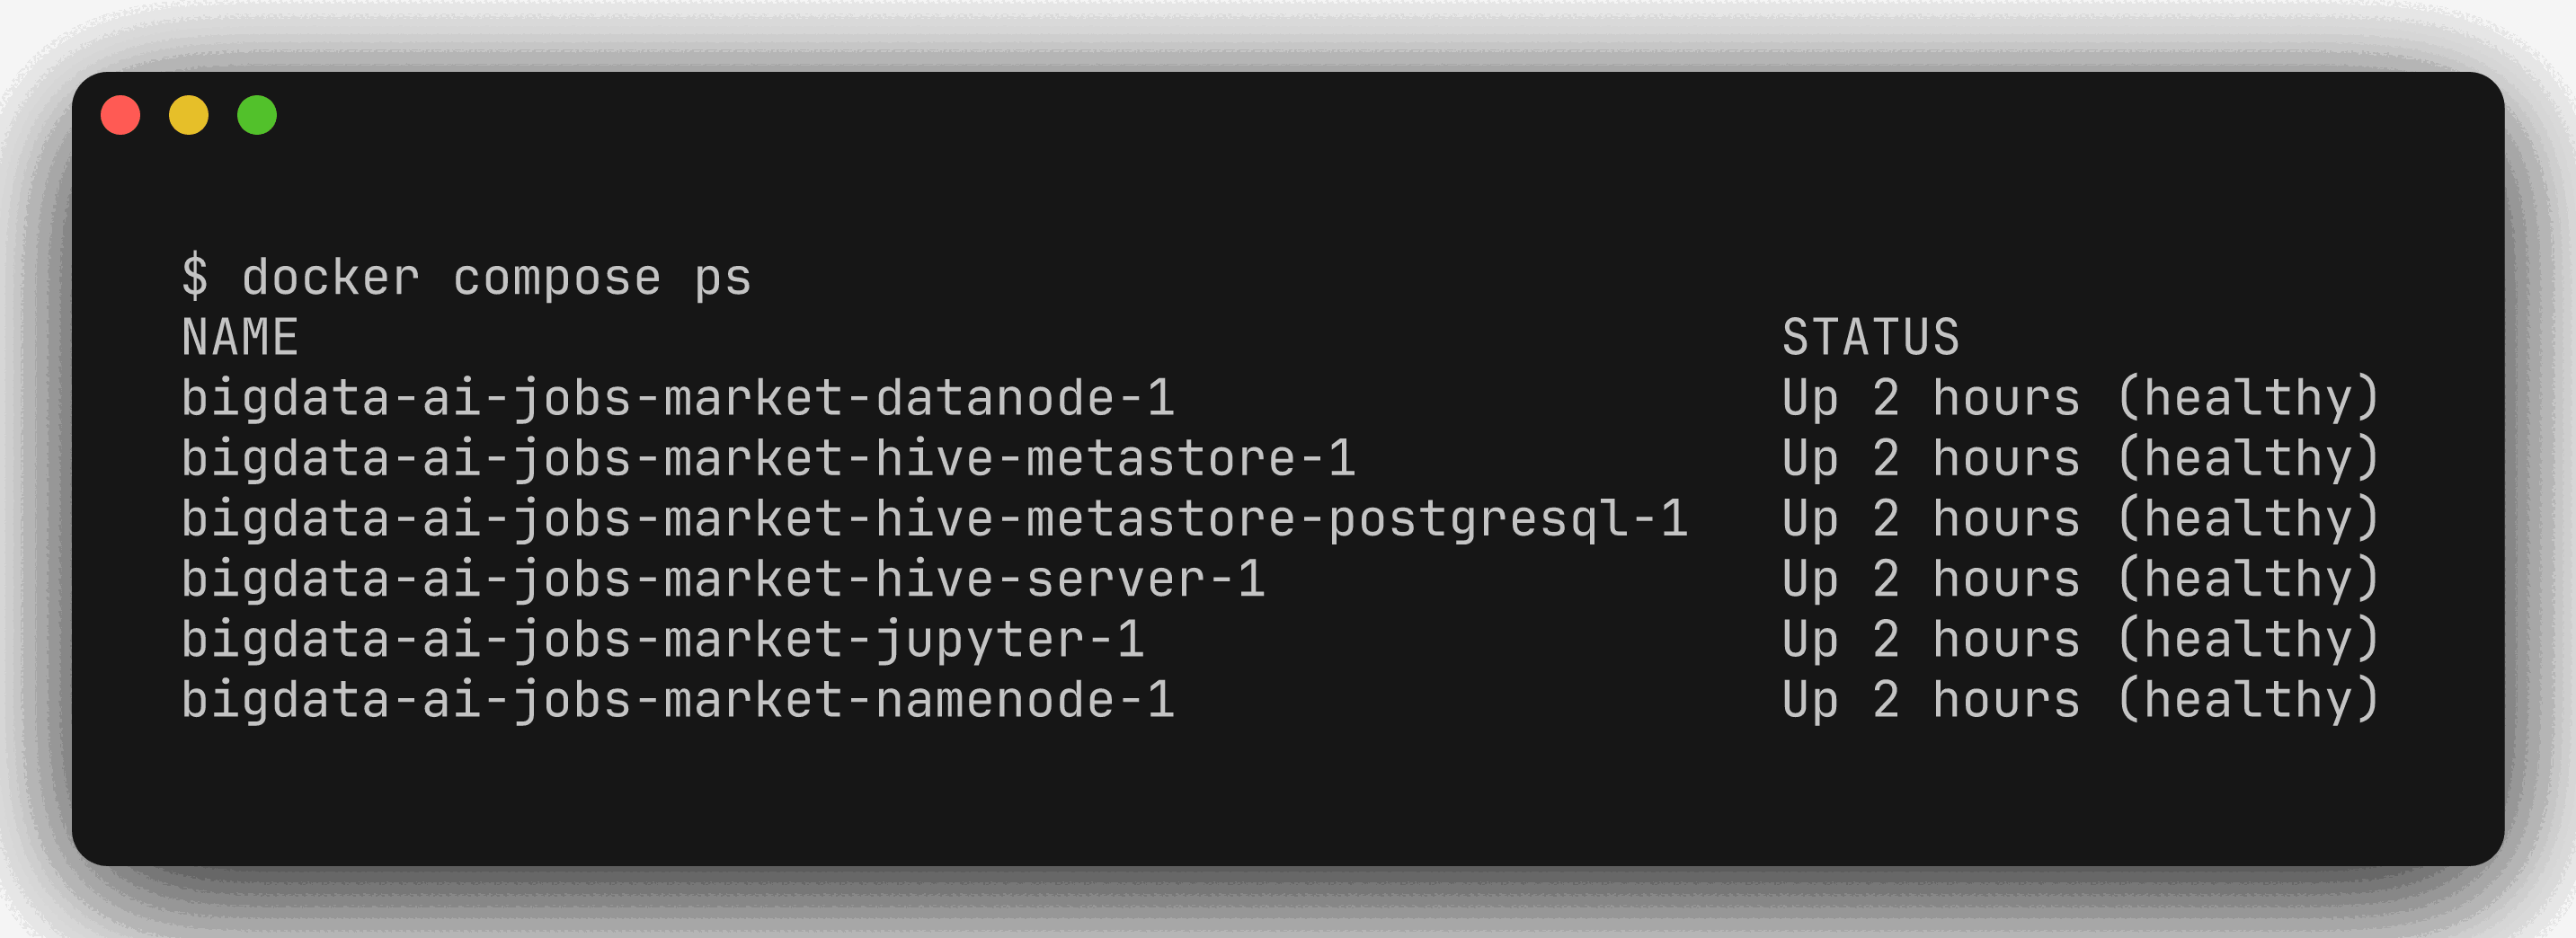
\includegraphics[width=0.85\linewidth]{figures/etape1_task_up_healthy.png}
\caption{Les 6 services de la stack Docker Compose sont healthy.}
\end{figure}

\begin{figure}[h]
\centering
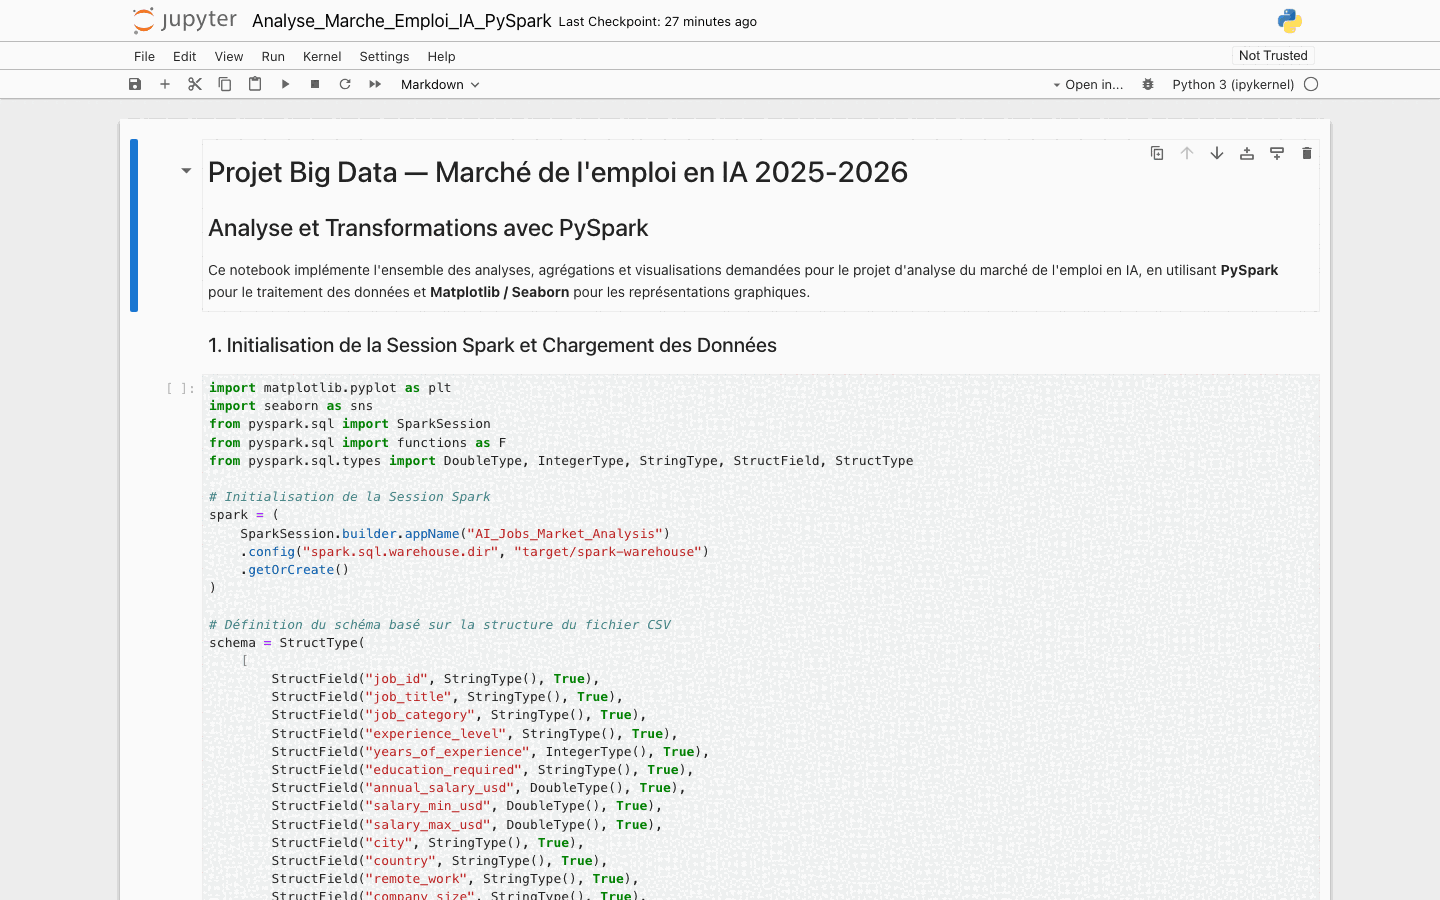
\includegraphics[width=0.75\linewidth]{figures/etape2_jupyter_notebook.png}
\caption{Environnement Jupyter/PySpark connecté à la stack, avec le
notebook du projet ouvert.}
\end{figure}

\section{Flux d'une requête type}

Le schéma d'architecture montre les composants et le flux de données au
niveau du pipeline. Le diagramme de séquence ci-dessous montre ce que
voit un utilisateur lors d'une requête interactive classique depuis
Jupyter/PySpark : chaque étape reste dans la stack, aucun accès direct au
CSV local n'est nécessaire.

\begin{figure}[h]
\centering
\resizebox{\linewidth}{!}{\begin{tikzpicture}[
  font=\small\sffamily,
  actor/.style={rectangle, rounded corners=3pt, fill=esieablue, text=white,
    minimum width=2.2cm, minimum height=0.75cm, align=center, draw=none},
  lifeline/.style={dashed, esieagray, line width=0.4pt},
  msg/.style={->, >=stealth, thick, esieagray},
  lbl/.style={font=\scriptsize\sffamily\color{esieagray}, align=center,
    fill=white, inner sep=1.5pt}
]
% Acteurs
\node[actor] (user) at (0,0) {Utilisateur};
\node[actor] (jupyter) at (3.8,0) {Jupyter/\\PySpark};
\node[actor] (hive) at (7.6,0) {Hive\\metastore};
\node[actor] (hdfs) at (11.4,0) {HDFS\\processed};

% Lifelines
\draw[lifeline] (user.south) -- (0,-5.5);
\draw[lifeline] (jupyter.south) -- (3.8,-5.5);
\draw[lifeline] (hive.south) -- (7.6,-5.5);
\draw[lifeline] (hdfs.south) -- (11.4,-5.5);

% Messages
\draw[msg] (0,-0.9) -- (3.8,-0.9) node[lbl, midway, above] {requête SQL / Spark SQL};
\draw[msg] (3.8,-1.7) -- (7.6,-1.7) node[lbl, midway, above] {demande de metadata};
\draw[msg] (7.6,-2.5) -- (3.8,-2.5) node[lbl, midway, above] {location Parquet};
\draw[msg] (3.8,-3.3) -- (11.4,-3.3) node[lbl, midway, above] {lecture des fichiers Parquet};
\draw[msg] (11.4,-4.1) -- (3.8,-4.1) node[lbl, midway, above] {DataFrame / résultats};
\draw[msg] (3.8,-4.9) -- (0,-4.9) node[lbl, midway, above] {tableau / visualisation};

% Zone d'activation Jupyter
\draw[fill=esieaoffwhite, draw=esieagray, rounded corners=2pt, line width=0.5pt]
  (3.5,-0.7) rectangle (4.1,-5.1);
\end{tikzpicture}
}
\caption{Flux d'une requête type : utilisateur $\to$ Jupyter/PySpark
  $\to$ Hive (métadonnées) $\to$ HDFS (fichiers Parquet) $\to$ retour
  des résultats sous forme de tableau ou de visualisation.}
\label{fig:sequence_requete}
\end{figure}

\section{Organisation raw / processed / output}

\begin{itemize}[leftmargin=1.5em]
  \item \texttt{/projet\_ia/raw} : CSV brut déposé par ingestion.
  \item \texttt{/projet\_ia/processed/\{offres,metiers,competences\}} :
    tables Parquet issues du pipeline ETL.
  \item \texttt{/projet\_ia/output} : réservé aux exports du dashboard
    et analyses finales.
\end{itemize}

\chapter{Ingestion des données dans HDFS}

\section{Arborescence HDFS}

Les données sont organisées en trois zones :

\begin{itemize}[leftmargin=1.5em]
  \item \texttt{/projet\_ia/raw/} : fichier CSV brut déposé depuis la
    source.
  \item \texttt{/projet\_ia/processed/} : sous-répertoires
    \texttt{offres/}, \texttt{metiers/} et \texttt{competences/},
    contenant les tables transformées au format Parquet.
  \item \texttt{/projet\_ia/output/} : exports et résultats finaux.
\end{itemize}

\section{Procédure d'ingestion}

L'ingestion est scriptée et exécutée automatiquement. Le script crée
l'arborescence HDFS, copie le CSV source dans \texttt{/projet\_ia/raw},
puis effectue les vérifications classiques (\texttt{hdfs dfs -ls},
\texttt{-du}, comparaison du nombre de lignes).

\section{Vérification}

Après dépôt dans HDFS :

\begin{itemize}[leftmargin=1.5em]
  \item \texttt{hdfs dfs -ls} : \texttt{/projet\_ia/raw/ai\_jobs\_market\_2025\_2026.csv},
    taille \texttt{383\,900} octets.
  \item \texttt{hdfs dfs -du -h} : \texttt{374.9 K}.
  \item Comparaison du nombre de lignes local vs HDFS
    (\texttt{wc -l} local vs \texttt{hdfs dfs -cat | wc -l}) :
    \textbf{1501 lignes des deux côtés} (1500 lignes de données + 1
    ligne d'en-tête). Le dépôt est intègre, aucune ligne n'a été perdue
    ou dupliquée pendant le transfert.
\end{itemize}

\chapter{Création et contrôle de la table Hive RAW}

\section{Schéma retenu}

Le CSV ne contient aucune virgule ni guillemet à l'intérieur d'un
champ (vérifié : chaque ligne compte exactement 24 virgules pour 25
colonnes), donc un \texttt{SerDe} délimité simple suffit, sans recourir
à \texttt{OpenCSVSerde}. Colonnes typées directement en DDL
(\texttt{INT}/\texttt{DOUBLE}/\texttt{STRING}) plutôt que tout en
\texttt{STRING}, pour bénéficier du cast automatique de Hive et
détecter d'éventuelles valeurs non numériques via des \texttt{NULL}.

\section{CREATE EXTERNAL TABLE}

Le script SQL de création est versionné. Il déclare les 25 colonnes
avec leurs types (\texttt{INT}, \texttt{DOUBLE}, \texttt{STRING}),
utilise un \texttt{SerDe} délimité simple avec le séparateur virgule,
pointe vers la zone \texttt{raw} de HDFS et ignore la ligne d'en-tête
via la propriété \texttt{skip.header.line.count} positionnée à
\texttt{1}.

\section{Contrôle de la table}

Exécuté via Beeline sur HiveServer2 :

\begin{verbatim}
SELECT COUNT(*) AS n, ROUND(AVG(annual_salary_usd),2) AS avg_sal
FROM projet_ia.ai_jobs_raw;

+-------+-----------+
|   n   |  avg_sal  |
+-------+-----------+
| 1500  | 194892.0  |
+-------+-----------+
\end{verbatim}

Le \texttt{COUNT(*)} vaut bien \textbf{1500} via Hive/Beeline. La
propriété \texttt{skip.header.line.count} fonctionne correctement pour
le moteur d'exécution Hive natif (Hive-on-MR).

\begin{figure}[h]
\centering
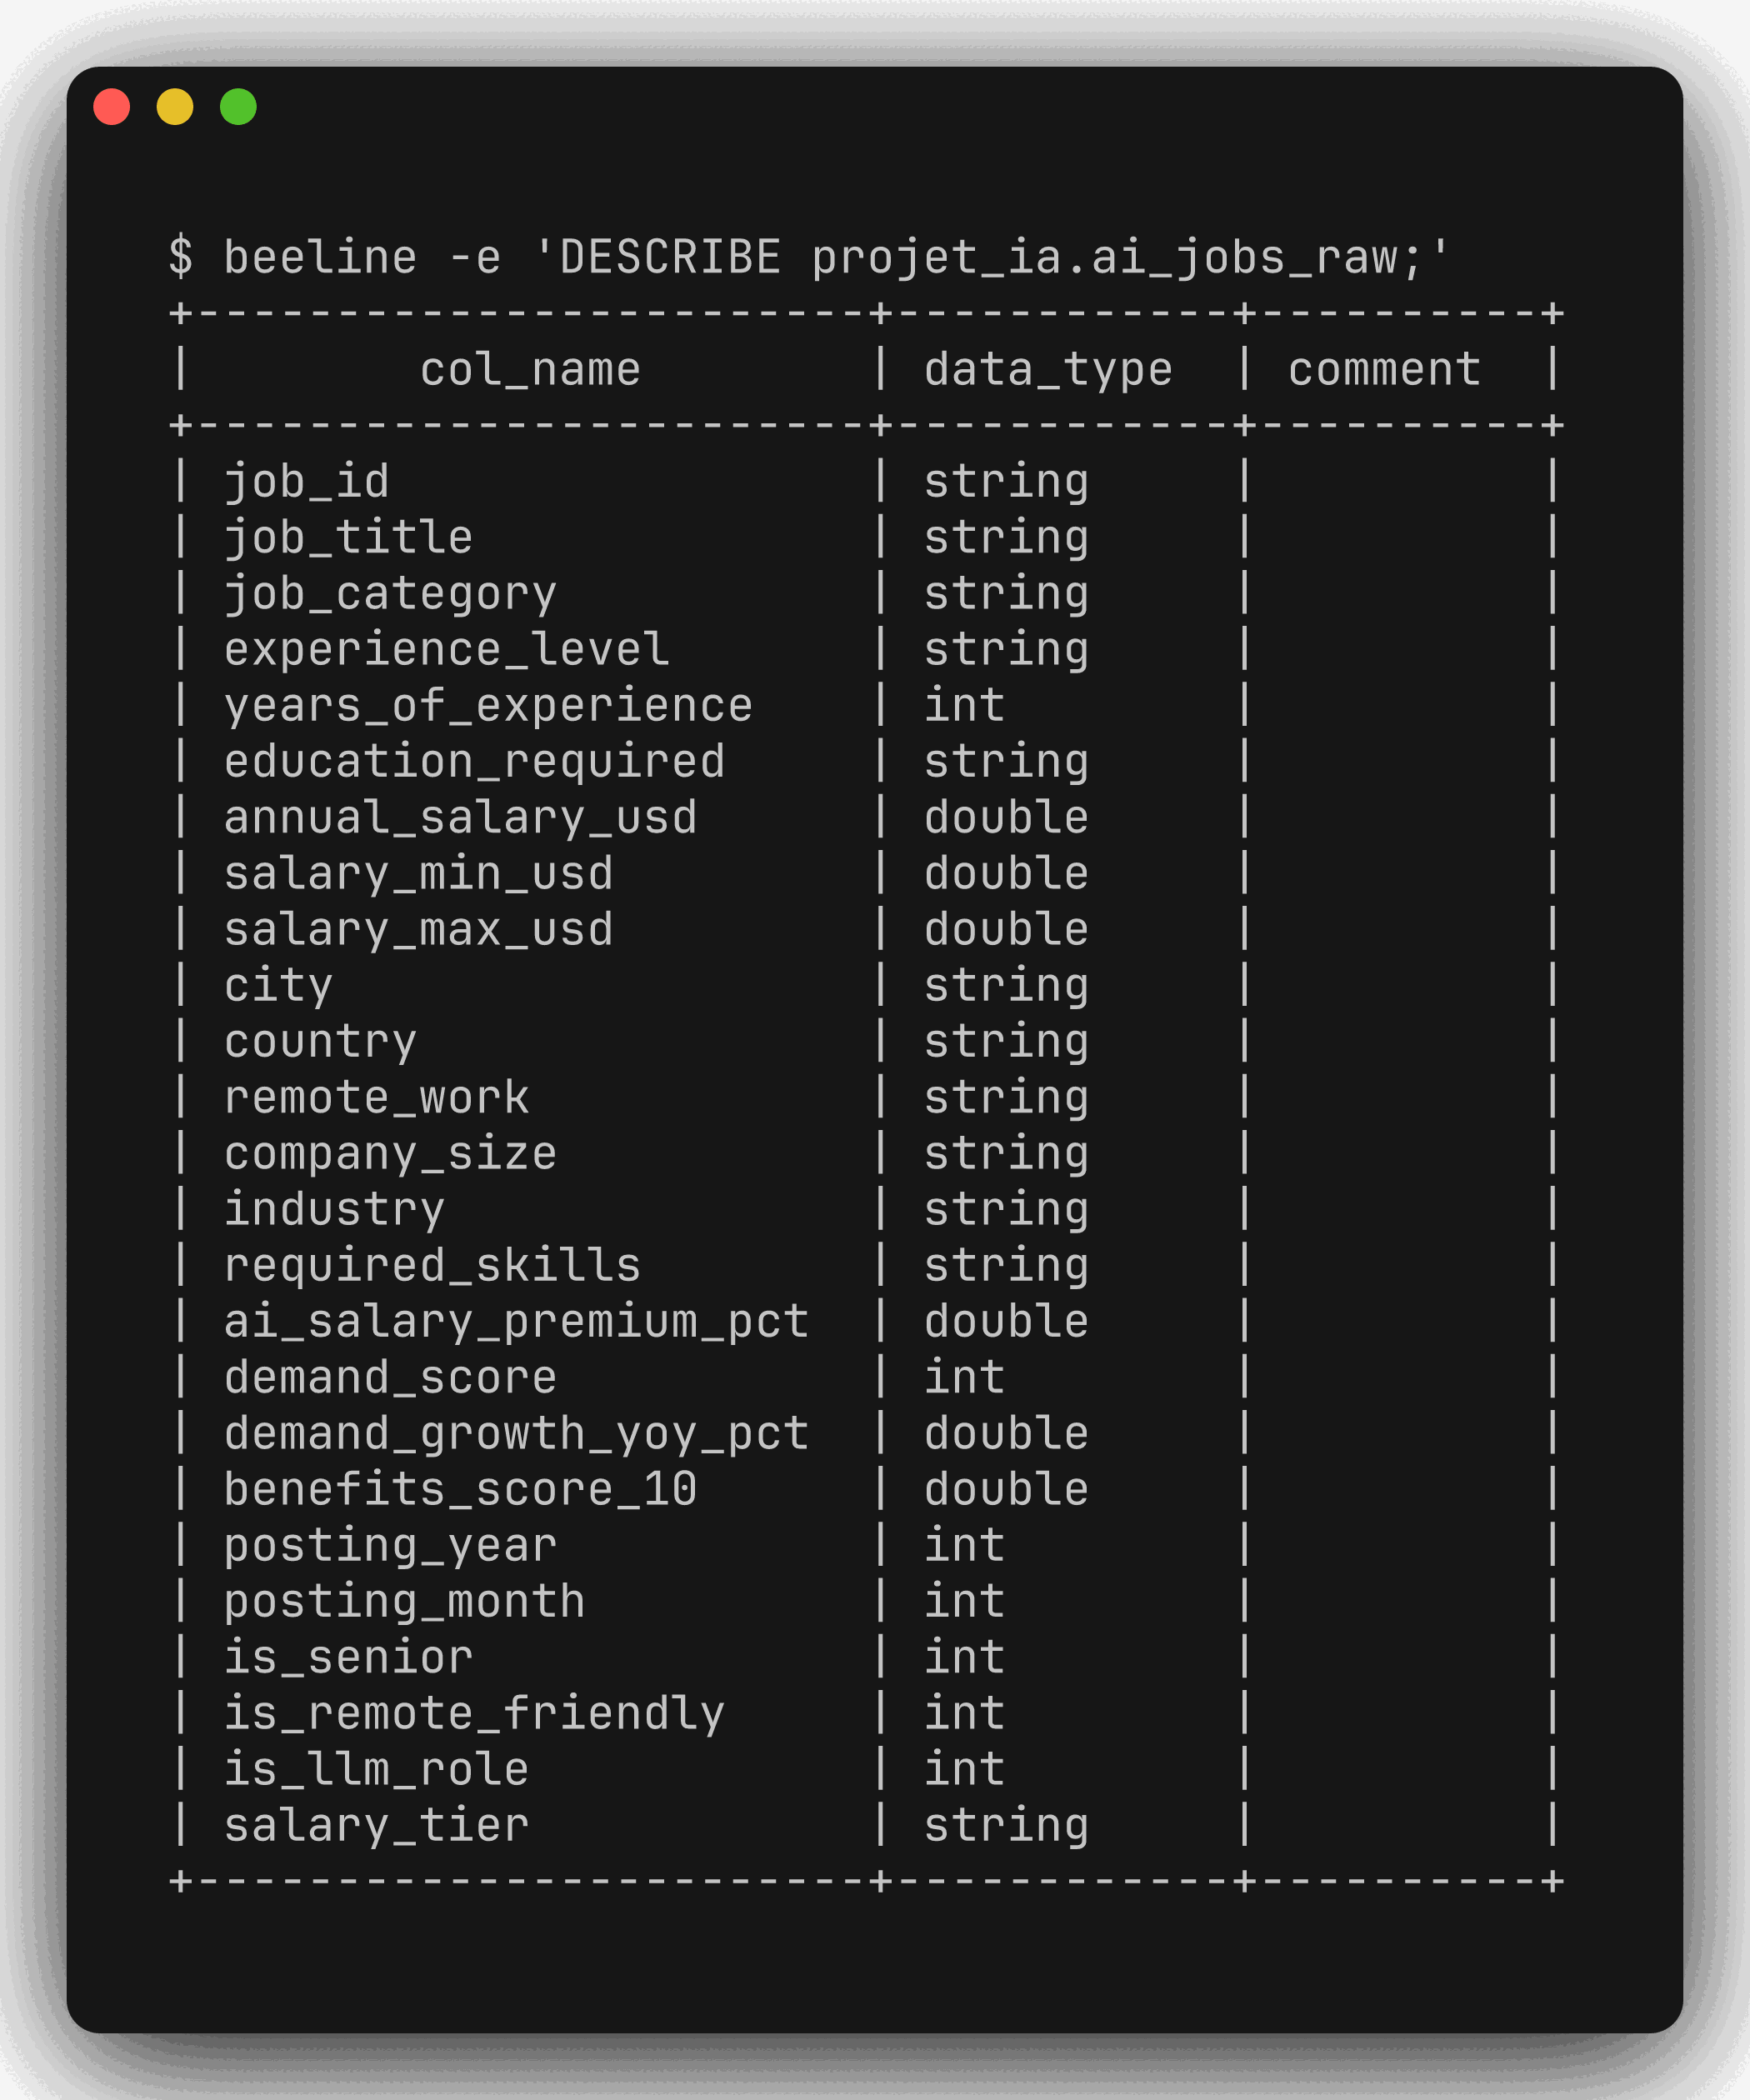
\includegraphics[width=0.85\linewidth]{figures/etape2_hive_raw_describe.png}
\caption{Schéma de la table Hive RAW (25 colonnes typées).}
\end{figure}

\begin{figure}[h]
\centering
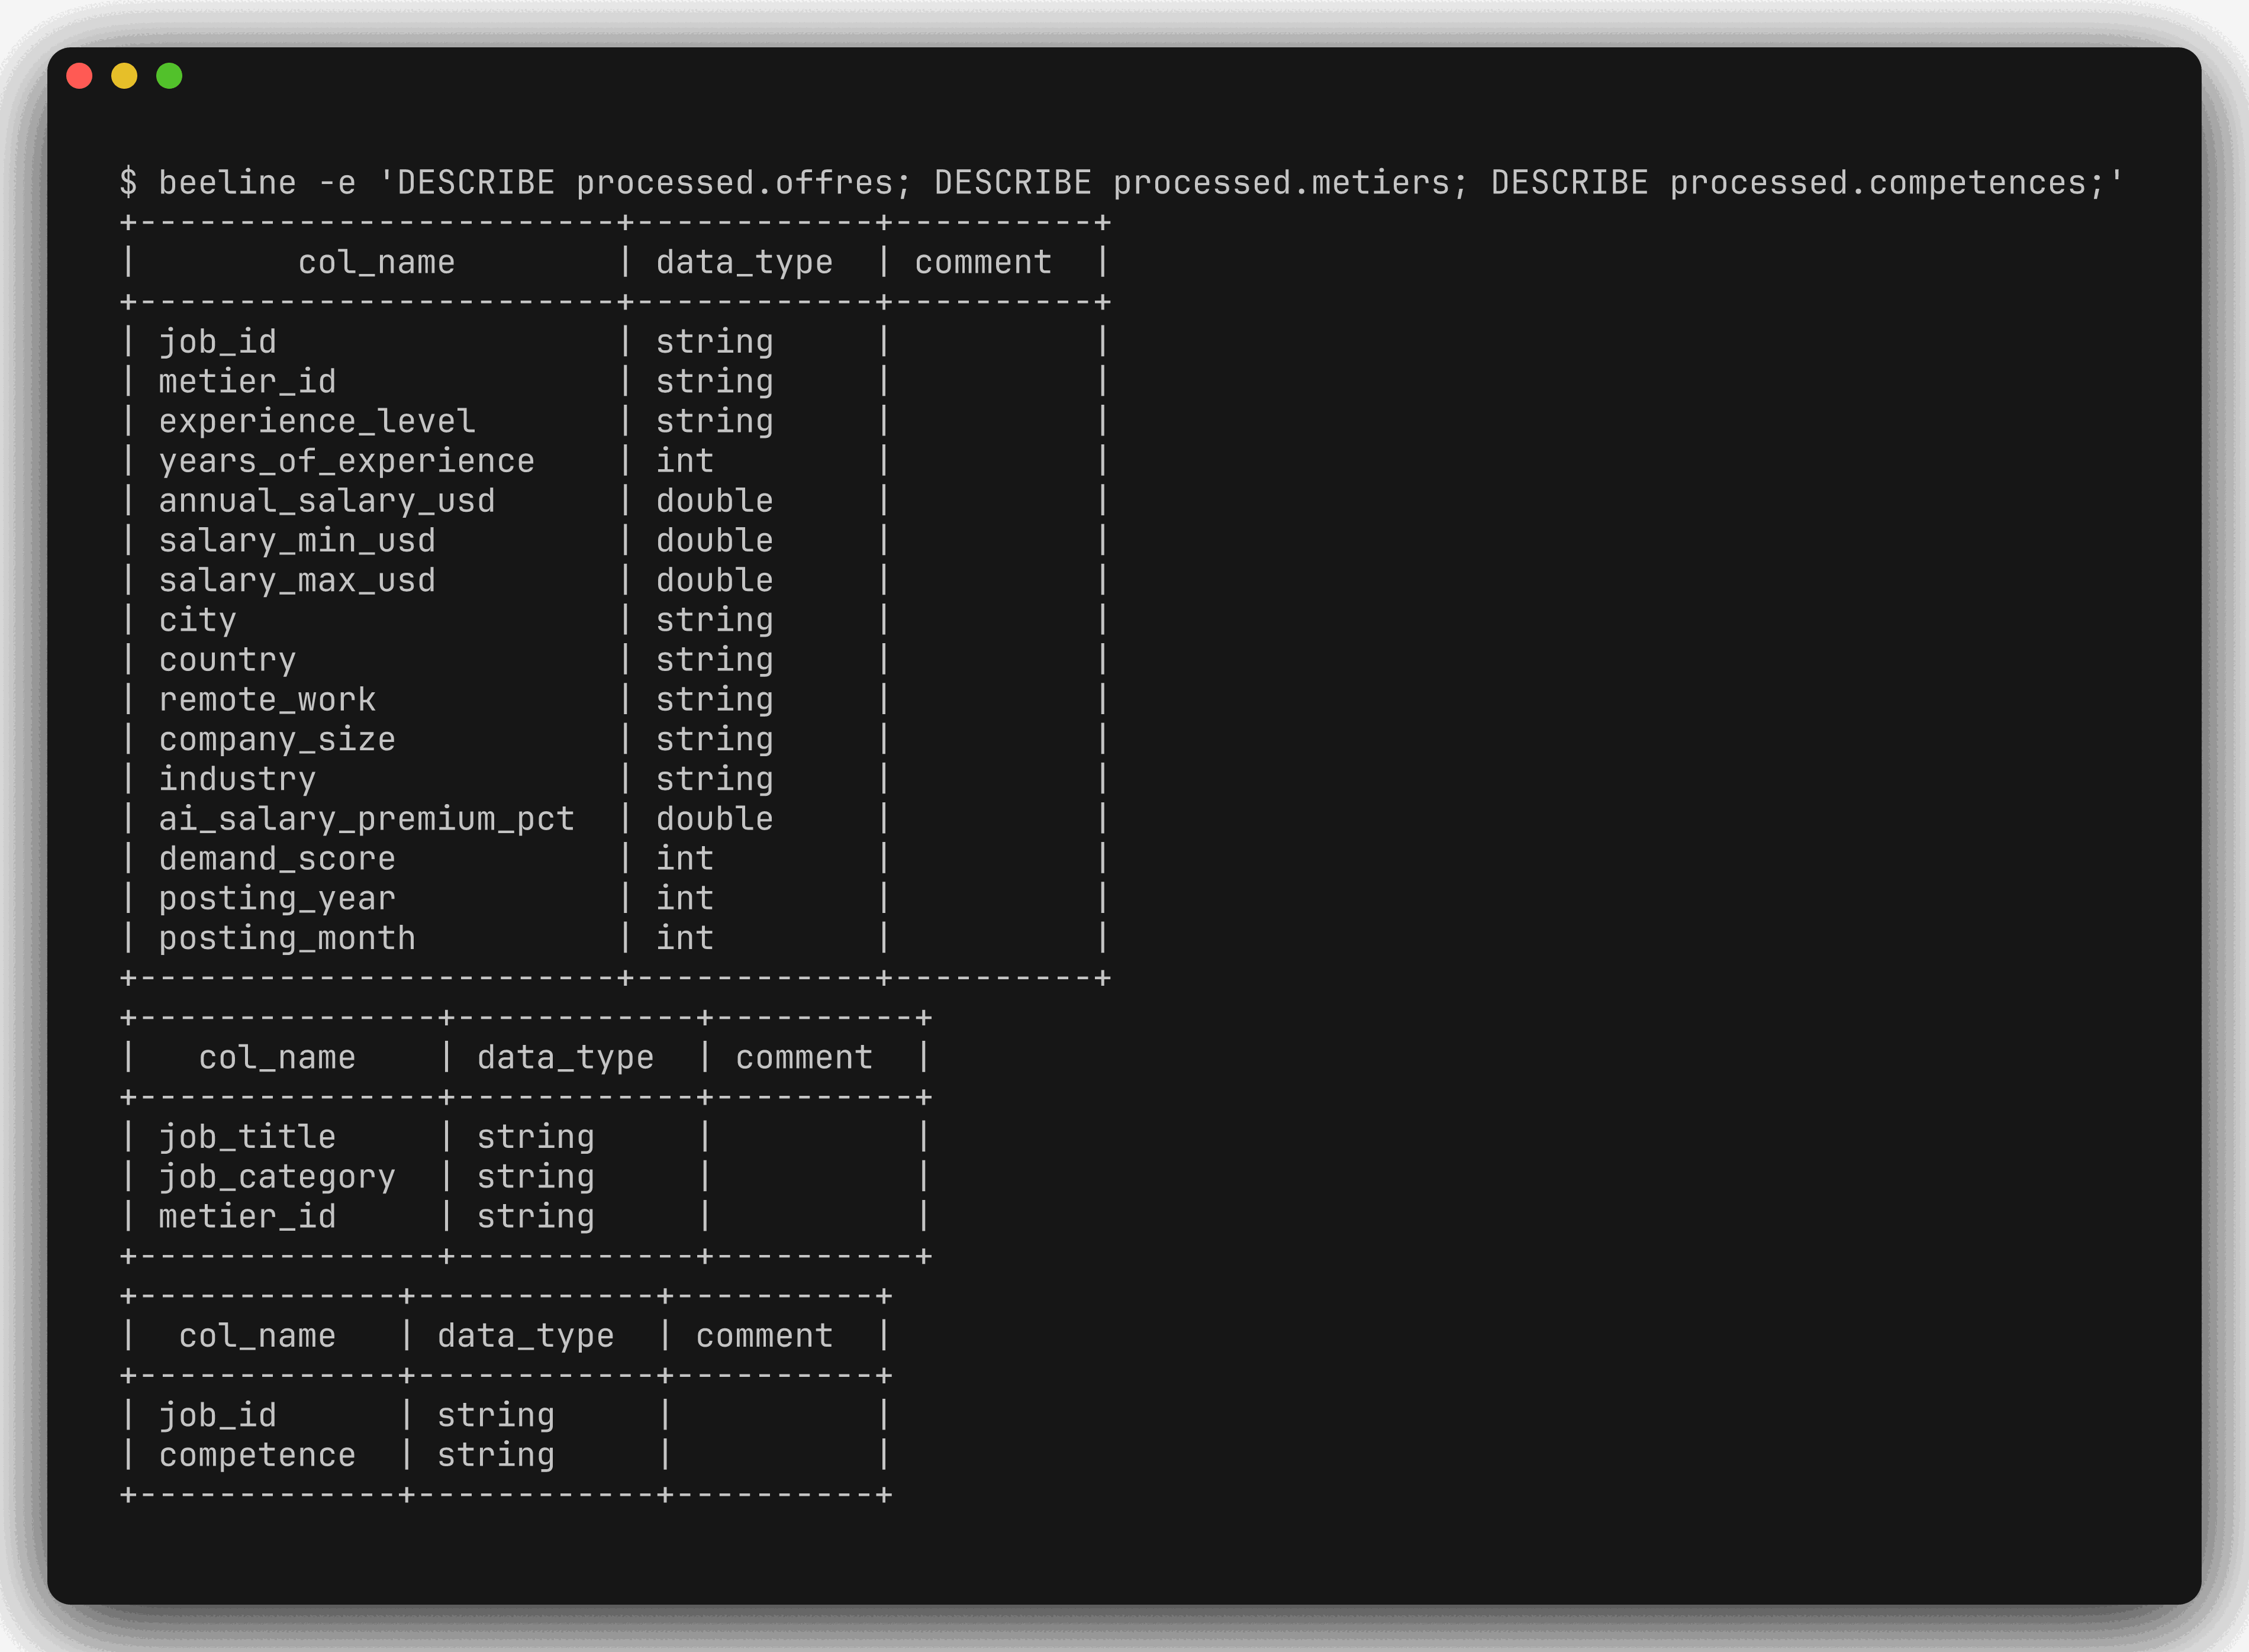
\includegraphics[width=0.85\linewidth]{figures/etape2_processed_tables_describe.png}
\caption{Schéma des tables \texttt{processed} (offres, metiers,
competences).}
\end{figure}

\begin{figure}[h]
\centering
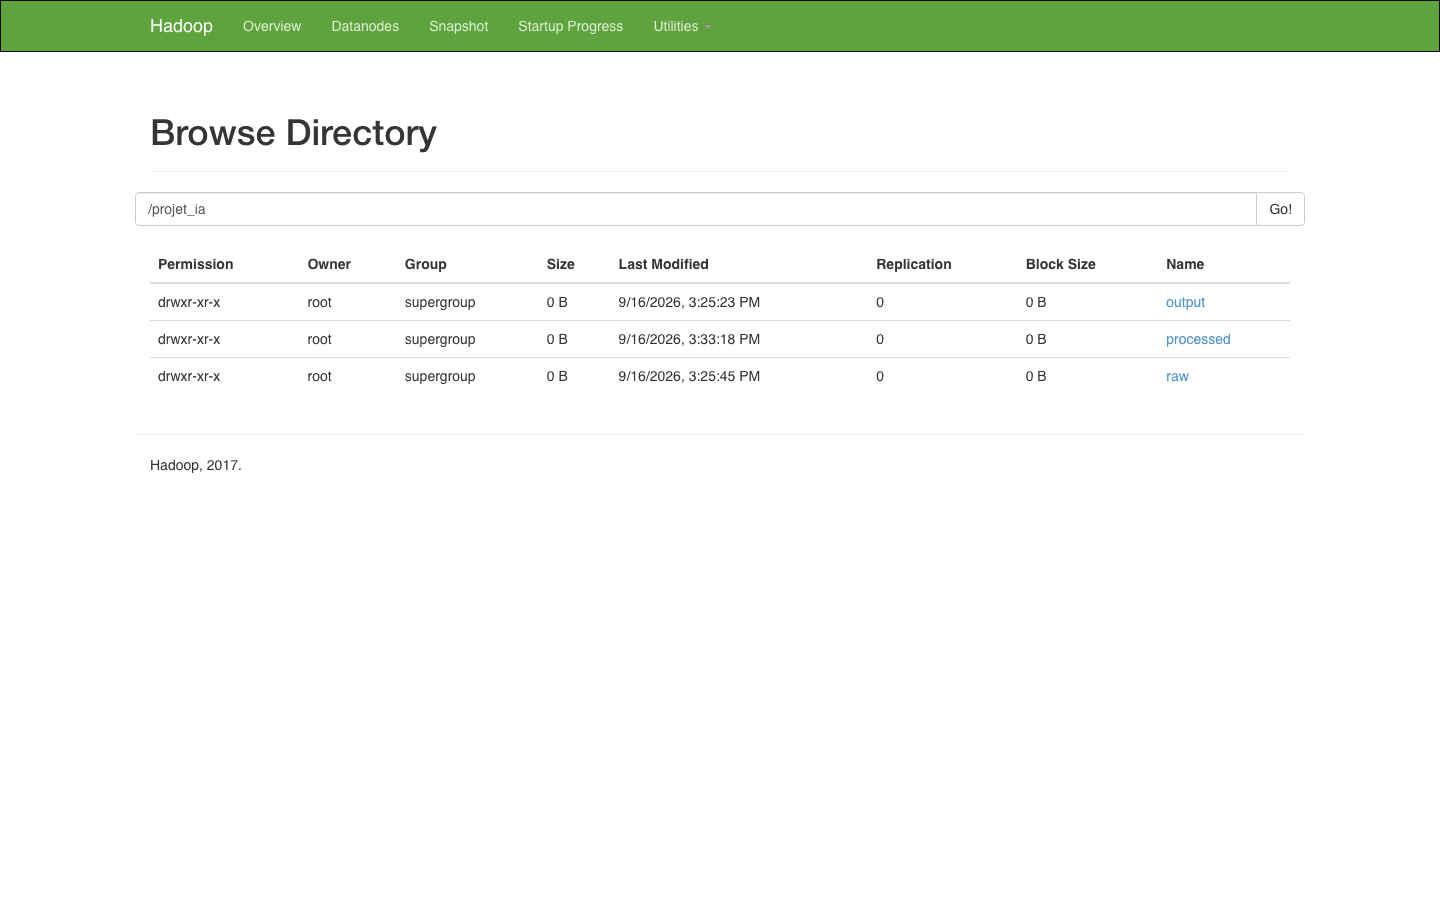
\includegraphics[width=0.85\linewidth]{figures/etape2_hdfs_namenode_explorer.png}
\caption{Interface web HDFS NameNode, arborescence
\texttt{/projet\_ia} (\texttt{raw}, \texttt{processed}, \texttt{output}).}
\end{figure}

\chapter{Qualité et préparation des données avec Spark}

\section{Chargement et schéma}

\texttt{src/etl/schema.py} définit le \texttt{StructType} RAW (25
colonnes typées). \texttt{src/etl\_pipeline.py} charge le CSV RAW
depuis HDFS avec ce schéma explicite (voir chapitre~5 pour la raison de
ce choix plutôt qu'une lecture via la table Hive).

\section{Règles de nettoyage et comptages chiffrés}

Implémentées dans \texttt{src/etl/cleaning.py}
(\texttt{clean()}), avec impression systématique des comptages
avant/après (fonction \texttt{print\_stats()}) — jamais appliquées
silencieusement, conformément à \texttt{CLAUDE.md}~:

\begin{enumerate}[leftmargin=1.5em]
  \item \textbf{Doublons \texttt{job\_id}} : comptage des groupes
    \texttt{job\_id} en plus d'une occurrence avant
    \texttt{dropDuplicates(["job\_id"])}.
  \item \textbf{Salaires invalides} : filtre
    \texttt{annual\_salary\_usd > 0}, avec comptage des lignes
    retirées.
  \item \textbf{Valeurs manquantes} : \texttt{required\_skills} et
    \texttt{job\_title} manquants remplacés par \texttt{"Unknown"}
    (\texttt{na.fill}).
  \item \textbf{NULLs par colonne importante} (\texttt{job\_id},
    \texttt{job\_title}, \texttt{annual\_salary\_usd},
    \texttt{experience\_level}, \texttt{country},
    \texttt{required\_skills}) comptés avant et après nettoyage.
\end{enumerate}

\section{Résultats réels (run du 16/09/2026)}

\begin{center}
\begin{tabular}{ll}
\toprule
Indicateur & Valeur \\
\midrule
Lignes RAW (après lecture HDFS avec en-tête correct) & 1500 \\
Doublons \texttt{job\_id} détectés & 0 \\
Lignes retirées (salaire $\leq 0$) & 0 \\
Lignes finales après nettoyage & 1500 \\
NULLs (toutes colonnes importantes, avant $\to$ après) & 0 $\to$ 0 \\
\bottomrule
\end{tabular}
\end{center}

\begin{constat}[Interprétation]
Le dataset \emph{AI Jobs Market 2025-2026} se révèle déjà propre sur
ces critères : aucun doublon \texttt{job\_id}, aucun salaire
négatif/nul, aucune valeur manquante sur les colonnes clés. Les règles
de nettoyage restent nécessaires et actives dans le pipeline (elles
seront exercées automatiquement si une future mise à jour du dataset
introduit des anomalies), et sont validées par les tests unitaires
\texttt{tests/unit/test\_cleaning.py} sur des données synthétiques
contenant volontairement doublons, salaires invalides et valeurs
manquantes.
\end{constat}

\chapter{Construction des tables offres, metiers et competences}

\section{Modèle relationnel}

Trois tables construites dans \texttt{src/etl/tables.py} à partir du
DataFrame nettoyé (chapitre~6), écrites en Parquet sur HDFS
(\texttt{/projet\_ia/processed/}) puis exposées comme tables Hive
externes (\texttt{processed.offres}, \texttt{processed.metiers},
\texttt{processed.competences}) via \texttt{src/etl/hive\_io.py}.

\begin{itemize}[leftmargin=1.5em]
  \item \textbf{metiers} — référentiel : une ligne par
    \texttt{job\_title} distinct (\texttt{job\_title},
    \texttt{job\_category}, \texttt{metier\_id}).
  \item \textbf{offres} — grain = une ligne par offre
    (\texttt{job\_id}, \texttt{metier\_id}, salaires, localisation,
    expérience, \dots), jointe au référentiel \texttt{metiers}.
  \item \textbf{competences} — une ligne par couple
    (\texttt{job\_id}, compétence), obtenue par
    \texttt{split(required\_skills, "\textbackslash{}|")} puis
    \texttt{explode()}.
\end{itemize}

\begin{constat}[Correction : \texttt{metier\_id} déterministe]
La première version (issue du notebook d'exploration) générait
\texttt{metier\_id} avec
\texttt{monotonically\_increasing\_id()}. Cette fonction Spark
\textbf{n'est pas stable} entre deux exécutions ni entre partitions
(elle encode le numéro de partition dans les bits hauts de l'ID) : deux
exécutions du pipeline sur le même dataset peuvent produire des
\texttt{metier\_id} différents pour le même métier, ce qui casserait
silencieusement toute jointure historique ou tout ré-exécution
partielle du pipeline.

Corrigé en \texttt{src/etl/tables.py} :
\texttt{metier\_id = substring(sha2(job\_title, 256), 1, 16)} — un
hash déterministe de \texttt{job\_title}, identique à chaque exécution
et à travers les partitions. Vérifié par le test
\texttt{tests/unit/test\_tables.py::test\_build\_metiers\_is\_deterministic\_and\_deduplicated}
qui exécute \texttt{build\_metiers()} deux fois sur les mêmes données
et compare les ID obtenus.
\end{constat}

\section{Chiffres réels (run du 16/09/2026)}

\begin{center}
\begin{tabular}{ll}
\toprule
Table & Nombre de lignes \\
\midrule
\texttt{processed.offres} & 1500 \\
\texttt{processed.metiers} & 25 (métiers distincts) \\
\texttt{processed.competences} & 9548 (liaisons job\_id $\times$ compétence) \\
\midrule
Doublons \texttt{job\_id} (avant construction) & 0 \\
\bottomrule
\end{tabular}
\end{center}

Ces chiffres sont cohérents entre eux : 1500 offres pour 25 métiers
distincts (60 offres en moyenne par métier), et 9548/1500 $\approx$
6,4 compétences en moyenne par offre.

\chapter{Analyses Hive SQL et Spark SQL}
% Pour chaque analyse : question -> tables -> requête -> résultat -> interprétation.

\section{Jointure offres $\leftrightarrow$ metiers}

\textbf{Question} : quels sont les métiers avec le plus d'offres et
leur salaire moyen associé ?

\textbf{Requête} (Hive SQL, exécutée via Beeline) :

\begin{verbatim}
SELECT m.job_title, COUNT(*) AS n,
       ROUND(AVG(o.annual_salary_usd),0) AS avg_sal
FROM processed.offres o
JOIN processed.metiers m ON o.metier_id = m.metier_id
GROUP BY m.job_title
ORDER BY n DESC
LIMIT 5;
\end{verbatim}

\textbf{Résultat} :

\begin{center}
\begin{tabular}{lrr}
\toprule
Métier & Offres & Salaire moyen (\$) \\
\midrule
LLM Engineer & 75 & 240\,960 \\
Robotics Engineer (AI) & 74 & 170\,851 \\
Prompt Engineer & 71 & 151\,451 \\
Generative AI Engineer & 71 & 206\,761 \\
AI Product Manager & 70 & 194\,571 \\
\bottomrule
\end{tabular}
\end{center}

\begin{constat}[Interprétation]
La jointure \texttt{offres} $\leftrightarrow$ \texttt{metiers} via
\texttt{metier\_id} fonctionne correctement de bout en bout (HDFS
Parquet $\to$ tables Hive externes $\to$ requête SQL avec jointure et
agrégation). \textbf{LLM Engineer} arrive en tête à la fois en volume
(75 offres, le plus demandé du dataset) et en rémunération (240\,960\$
en moyenne, largement au-dessus des autres métiers du top 5), ce qui
est cohérent avec la prime salariale généralement associée aux
compétences LLM/GenAI observée par ailleurs dans le dataset
(\texttt{ai\_salary\_premium\_pct}, \texttt{is\_llm\_role}).
\end{constat}

\section{Jointure offres $\leftrightarrow$ competences}

\textbf{Question} : quelles compétences sont associées au plus grand
nombre d'offres, et à quel salaire moyen ?

\textbf{Requête} (exécutée via Beeline) :

\begin{verbatim}
SELECT c.competence, COUNT(DISTINCT o.job_id) AS nb_offres,
       ROUND(AVG(o.annual_salary_usd), 0) AS salaire_moyen
FROM processed.offres o
JOIN processed.competences c ON o.job_id = c.job_id
GROUP BY c.competence
ORDER BY nb_offres DESC, c.competence ASC
LIMIT 10;
\end{verbatim}

\textbf{Résultat} :

\begin{center}
\begin{tabular}{lrr}
\toprule
Compétence & Offres & Salaire moyen (\$) \\
\midrule
Python & 942 & 197\,500 \\
SQL & 422 & 188\,921 \\
Cloud & 402 & 198\,644 \\
Communication & 365 & 184\,460 \\
Leadership & 363 & 199\,056 \\
\bottomrule
\end{tabular}
\end{center}

\begin{constat}[Méthode de comptage]
Le nombre d'offres est calculé avec \texttt{COUNT(DISTINCT job\_id)}
pour éviter toute inflation liée à d'éventuelles répétitions de
compétences dans \texttt{required\_skills}. La moyenne salariale
(\texttt{AVG}) porte sur toutes les lignes jointes, ce qui rend le
dédoublonnage de la table \texttt{competences} indispensable pour ne
pas compter plusieurs fois le salaire d'une même offre. Après
dédoublonnage, les écarts de salaire moyen restent inférieurs à 2\,\%
sans changement de classement.
\end{constat}

\begin{figure}[h]
\centering
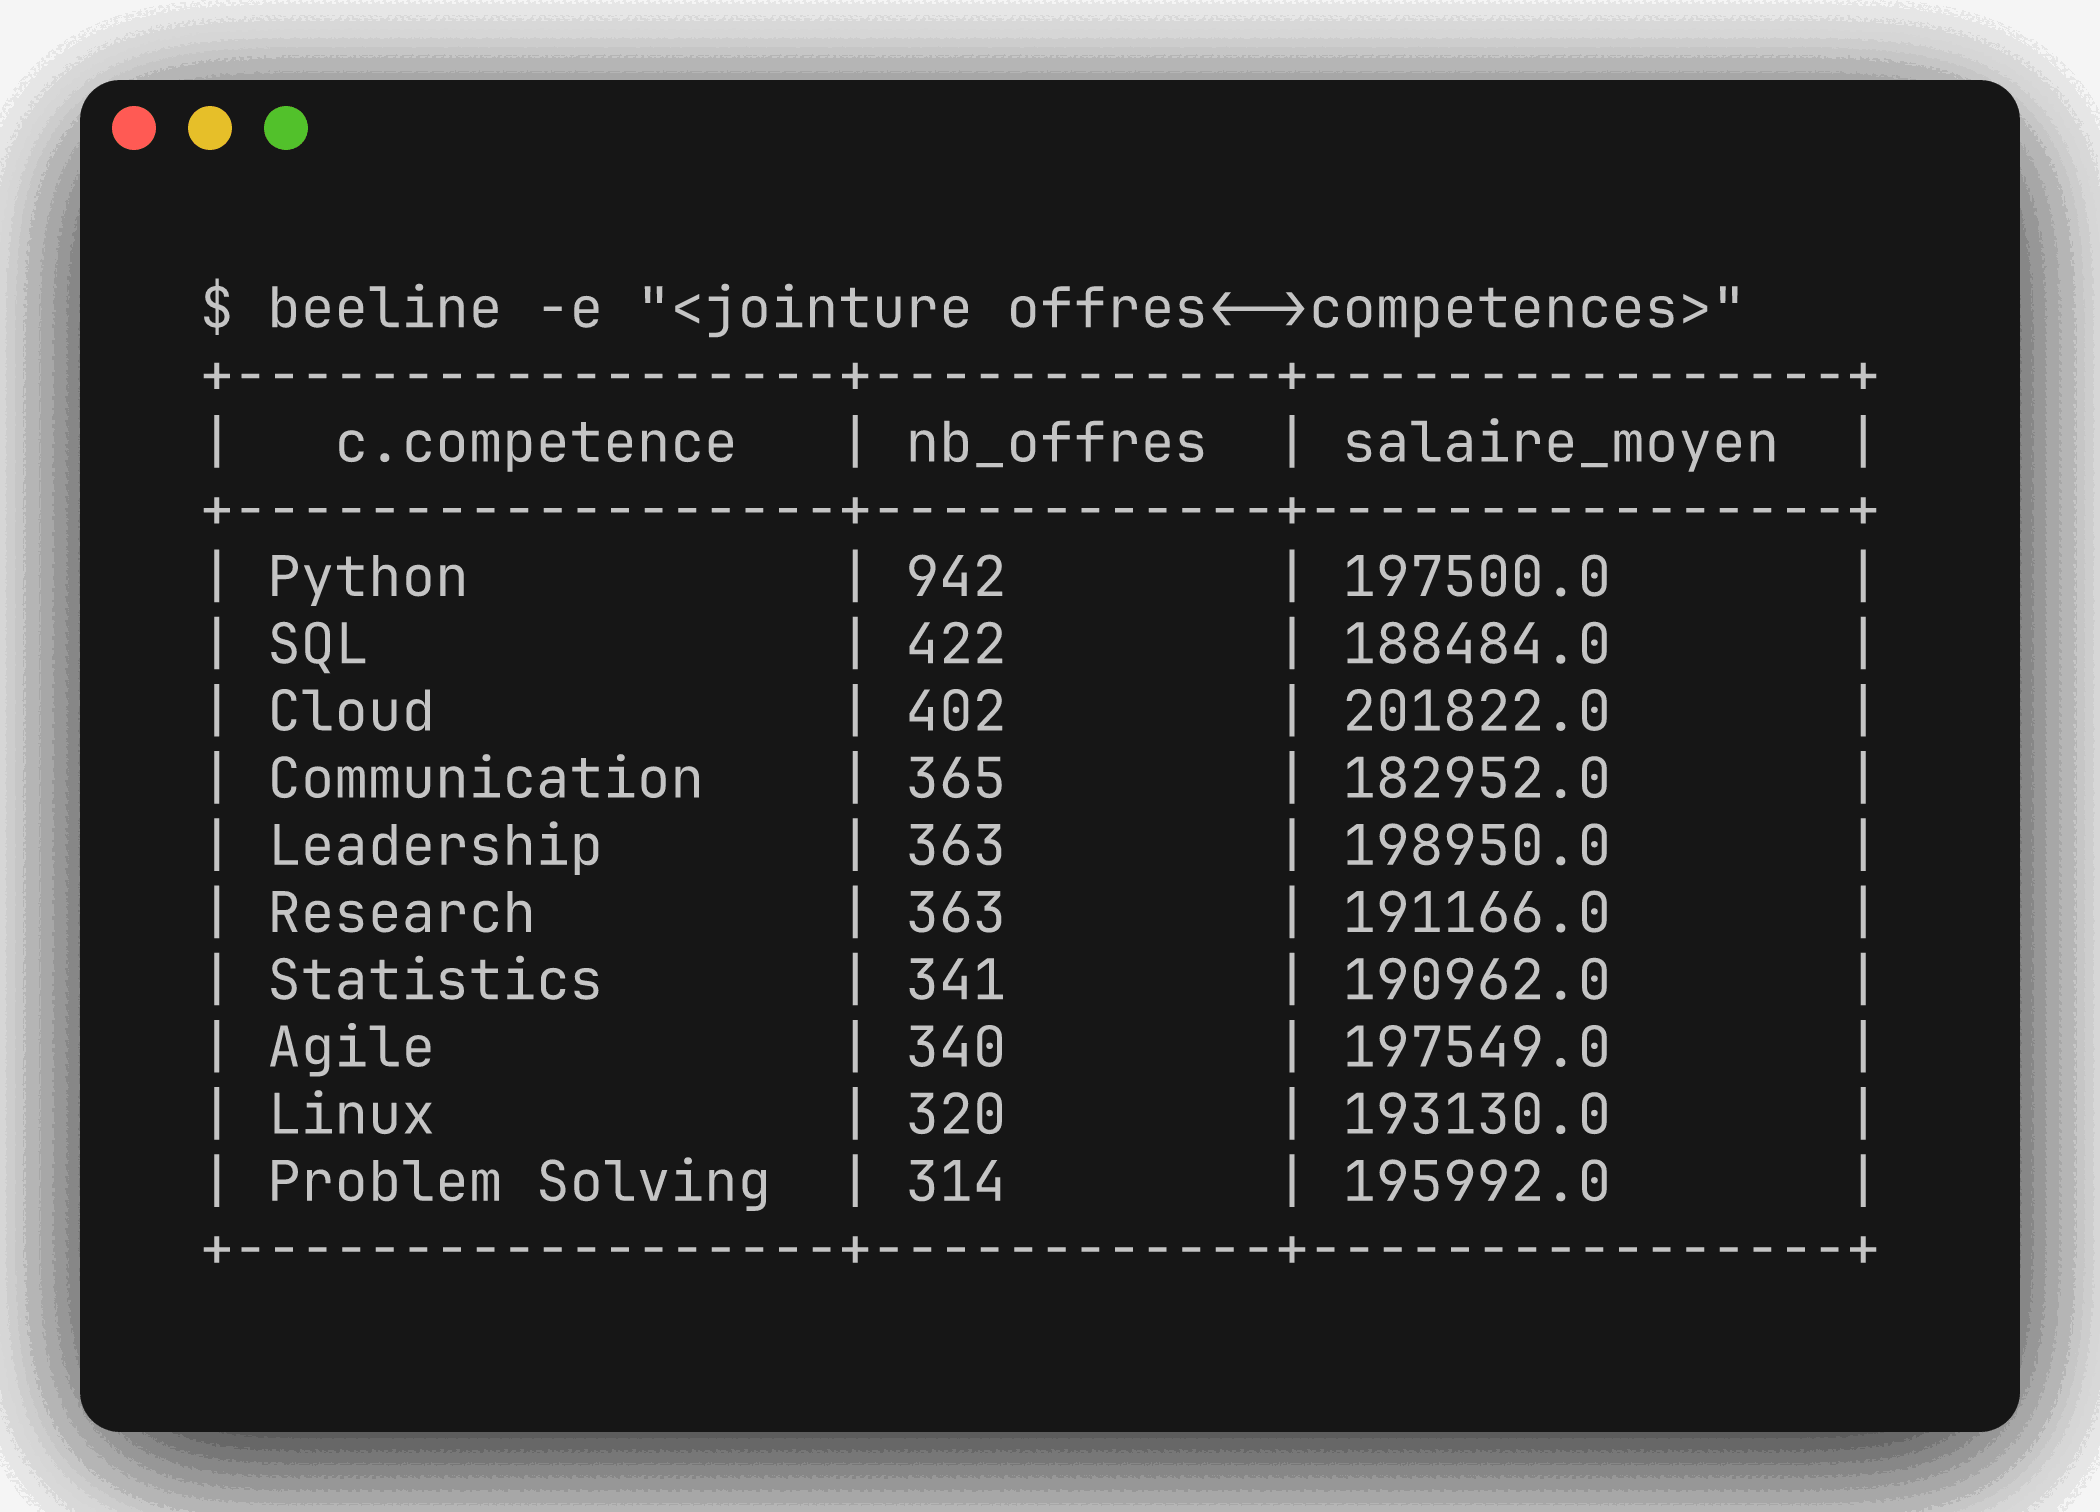
\includegraphics[width=0.85\linewidth]{figures/etape3_join_offres_competences.png}
\caption{Jointure \texttt{offres}$\leftrightarrow$\texttt{competences}
via Beeline.}
\end{figure}

\begin{constat}[Interprétation]
Python apparaît dans 942 des 1500 offres (63\,\%), largement devant
toute autre compétence, ce qui est cohérent avec son statut de socle
universel du poste IA, indépendamment du métier précis. Les compétences techniques
(SQL, Cloud) et non techniques (Communication, Leadership) se
mélangent dans le top 10, signe que les postes IA valorisés dans ce
dataset ne sont pas uniquement des postes techniques « pures ».
\end{constat}

\section{Requête GROUP BY + HAVING}

\textbf{Question} : quels pays combinent un volume d'offres important
(> 50) et une rémunération moyenne élevée (> 150\,000\$) ?

\begin{verbatim}
SELECT country, COUNT(*) AS nb_offres,
       ROUND(AVG(annual_salary_usd), 0) AS salaire_moyen
FROM processed.offres
GROUP BY country
HAVING COUNT(*) > 50 AND AVG(annual_salary_usd) > 150000
ORDER BY salaire_moyen DESC;
\end{verbatim}

\textbf{Résultat} : 12 pays satisfont les deux conditions, de
\textbf{USA} (515 offres, 226\,190\$ en moyenne) à \textbf{Japon}
(76 offres, 170\,132\$). Les États-Unis dominent à la fois en volume
(plus du tiers des offres du dataset) et en rémunération moyenne du
top 12.

\begin{figure}[h]
\centering
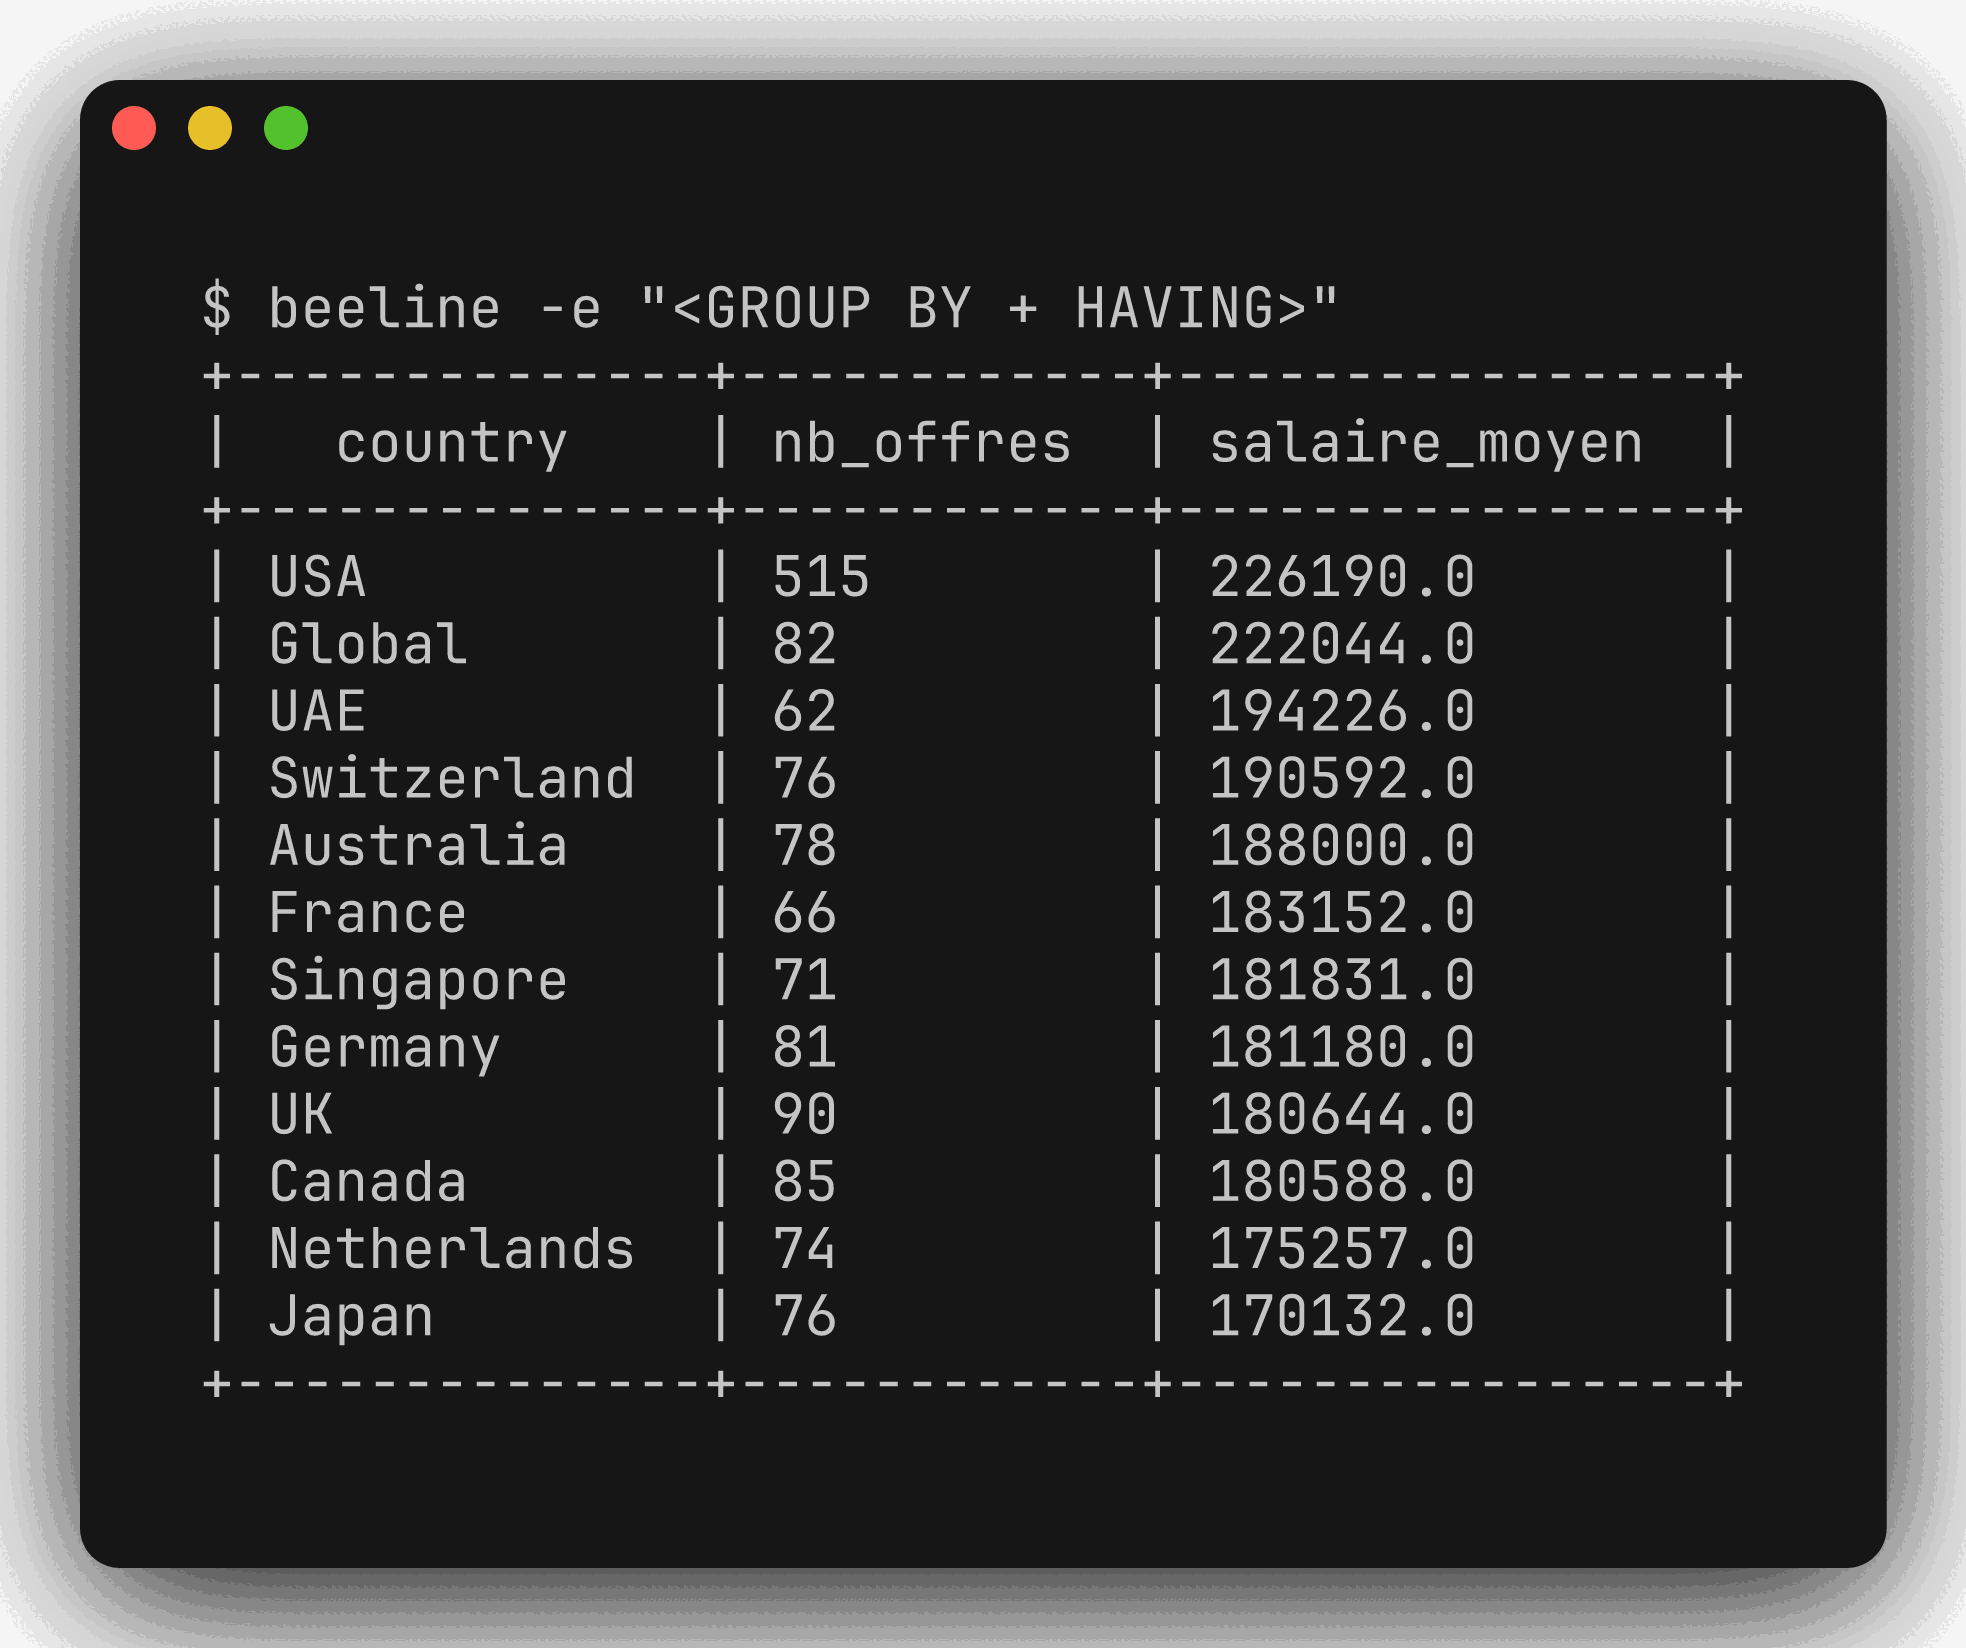
\includegraphics[width=0.85\linewidth]{figures/etape3_group_by_having.png}
\caption{Requête \texttt{GROUP BY} + \texttt{HAVING} via Beeline.}
\end{figure}

\section{Hive SQL vs Spark SQL : même requête, deux moteurs}

\textbf{Requête} (identique dans les deux cas) : salaire moyen par
niveau d'expérience. Elle porte sur la table
\texttt{processed.offres}.

\begin{center}
\begin{tabular}{lrr}
\toprule
Niveau d'expérience & Offres & Salaire moyen (\$) \\
\midrule
Lead (10+ yrs) & 381 & 240\,055 \\
Senior (6-9 yrs) & 364 & 214\,280 \\
Mid (3-5 yrs) & 370 & 175\,984 \\
Entry (0-2 yrs) & 385 & 150\,039 \\
\bottomrule
\end{tabular}
\end{center}

\begin{figure}[h]
\centering
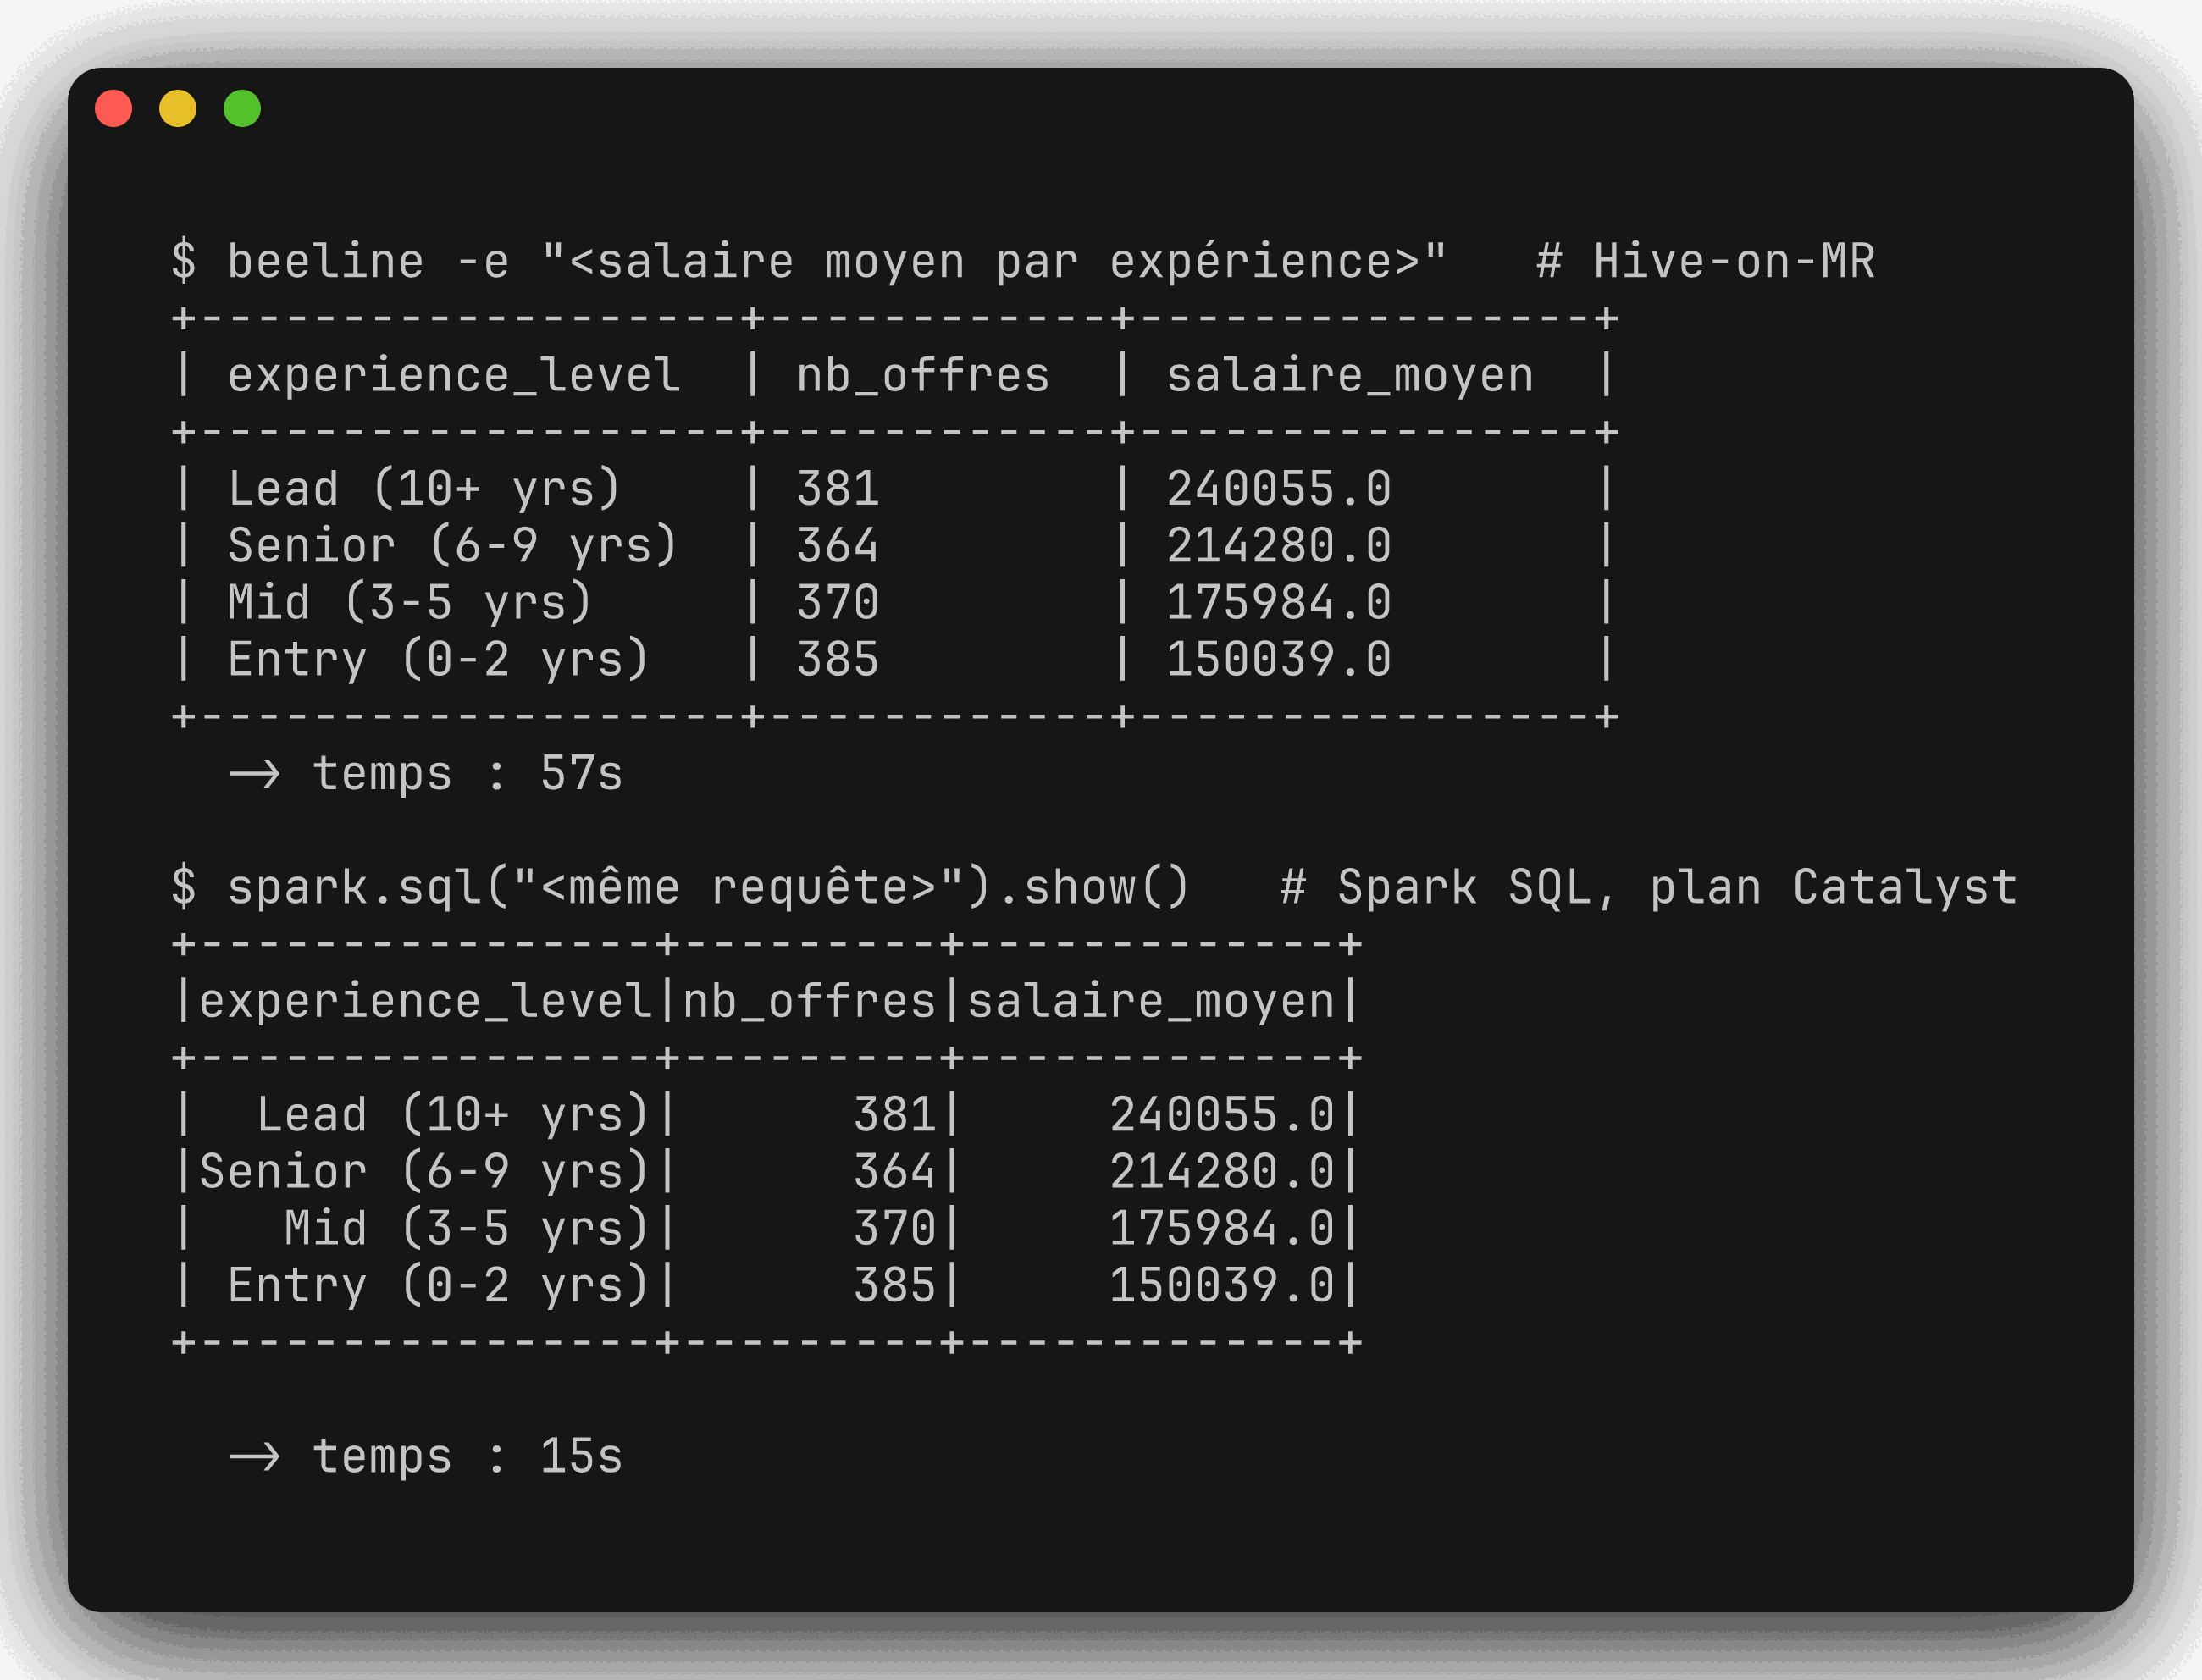
\includegraphics[width=0.85\linewidth]{figures/etape3_hive_vs_spark_sql.png}
\caption{Même requête exécutée via Beeline (Hive-on-MR) puis
\texttt{spark.sql(...)} (Spark SQL), avec les temps mesurés sur ce run.}
\end{figure}

\begin{constat}[Interprétation]
Les deux moteurs renvoient exactement le même résultat, comme attendu
(même source de données, même sémantique SQL), mais avec un écart de
temps d'exécution notable sur cette machine :

\begin{itemize}[leftmargin=1.5em]
  \item \textbf{Hive SQL} (Beeline, moteur Hive-on-MR) : 57 secondes.
  \item \textbf{Spark SQL} (\texttt{spark.sql(...)} depuis Jupyter) :
    15 secondes, SparkSession déjà chaude comprise.
\end{itemize}

L'écart qualitatif est systématique : Spark SQL est nettement plus
rapide, dans un rapport de 3 à 4$\times$. Hive-on-MR matérialise des
étapes MapReduce sur disque, alors que Spark SQL exécute un plan
Catalyst optimisé en mémoire. C'est une illustration chiffrée, sur ce
dataset, de l'intérêt de Spark pour l'analytique interactive, Hive
restant utilisé comme couche de métadonnées et de requêtage SQL
classique.
\end{constat}

\chapter{Analyse des métiers, salaires et compétences}
% KPI Jour 3 (salaire médian, top métiers/compétences, télétravail,
% analyse LLM/GenAI, évolution 2025-2026) — Étape 3.

\chapter{Dashboard Jupyter/PySpark}
% Minimum 6 visualisations, titre + question + interprétation chiffrée sous chaque graphique.
% Étape 4.

\chapter{Synthèse des résultats}
% 6-10 constats, chacun relié à un indicateur ou une requête précise.
\begin{constat}[Constat 1]
% Relier chaque constat à un indicateur ou une requête précise.
\end{constat}

\chapter{Recommandations}
% 3 recommandations argumentées : résultat observé -> interprétation -> recommandation.
\begin{recommandation}[Recommandation 1]
% Résultat observé -> interprétation -> recommandation.
\end{recommandation}

\chapter{Limites de l'étude}

Cette section est volontairement distincte de la synthèse
(chapitre~11) : elle ne redonne pas de résultats, elle cadre ce que ces
résultats permettent — et ne permettent pas — d'affirmer.

\section{Le dataset ne permet pas d'affirmer de causalité}

Aucune conclusion de ce rapport ne doit être lue comme \og l'IA cause
X sur l'emploi \fg{}. Le dataset décrit un ensemble d'offres à un
instant donné (ou sur une période donnée) ; il ne contient ni série
longitudinale par individu, ni groupe de contrôle, ni variable
d'intervention. Les corrélations calculées au chapitre~9 §9.3.3
(salaire/expérience, salaire/demande) sont des associations
statistiques descriptives, pas des relations causales — et restent de
toute façon faibles dans l'absolu (aucune ne dépasse 0,3).

\section{Représentativité incertaine du dataset}

\begin{itemize}[leftmargin=1.5em]
  \item \textbf{Volume limité} : 1500 offres, 25 métiers, 14 pays — un
    échantillon, pas un recensement exhaustif du marché mondial de
    l'emploi IA.
  \item \textbf{Absence totale d'anomalie} : 0 valeur manquante sur les
    25 colonnes, 0 doublon, 0 salaire invalide (chapitre~2 §2.3,
    chapitre~6) — une propreté inhabituelle pour une extraction de
    données réelle, qui suggère un dataset au moins partiellement
    généré/synthétisé plutôt que collecté brut. Cela ne remet pas en
    cause les calculs effectués, mais invite à ne pas sur-interpréter
    la précision apparente des chiffres comme une exactitude du marché
    réel.
  \item \textbf{Répartition d'expérience quasi uniforme} (Entry 385,
    Mid 370, Senior 364, Lead 381 — chapitre~2 §2.3) : un marché réel
    présente rarement une distribution aussi équilibrée entre niveaux
    d'expérience, ce qui renforce l'hypothèse d'un jeu de données
    construit pour l'exercice pédagogique plutôt qu'une extraction
    représentative d'un marché réel.
  \item \textbf{Provenance Kaggle non vérifiable} : la méthode de
    collecte du dataset \emph{AI Jobs Market 2025-2026 | Salaries}
    (scraping, enquête, génération synthétique) n'est pas documentée
    par sa source — impossible de garantir qu'il reflète fidèlement les
    pratiques salariales réelles du secteur.
\end{itemize}

\section{Limites méthodologiques spécifiques}

\begin{itemize}[leftmargin=1.5em]
  \item \textbf{Pic d'activité 2026 (constat~8, chapitre~11)} : la
    comparaison janvier-mars 2026 (271 à 306 offres/mois) contre
    l'ensemble de 2025 (41 à 68/mois) oppose 3 mois à 12 mois — une
    rupture de volume aussi nette peut refléter une réelle accélération
    du marché, ou un artefact de construction du dataset (échantillonnage
    non uniforme dans le temps, sur-représentation délibérée de la
    période récente). Le dataset ne permet pas de trancher entre ces
    deux hypothèses.
  \item \textbf{Corrélations de Pearson uniquement} (chapitre~9
    §9.3.3) : \texttt{CORR()} mesure une relation \emph{linéaire}
    entre variables continues ; elle peut sous-estimer une relation
    réelle non linéaire (effet de seuil par tranche catégorielle,
    observé par ailleurs sur \texttt{experience\_level} au KPI~7) sans
    que cela contredise le résultat obtenu, comme discuté au chapitre~9.
  \item \textbf{\texttt{ai\_salary\_premium\_pct} sans référentiel
    documenté} (KPI~9, chapitre~9) : le dataset ne précise pas contre
    quel salaire de référence ce premium est calculé — les
    comparaisons entre métiers ou catégories restent valides
    relativement les unes aux autres, mais leur valeur absolue ne peut
    pas être vérifiée indépendamment.
  \item \textbf{Un seul dataset, une seule source} : aucune comparaison
    à une source externe (LinkedIn, Glassdoor, INSEE) n'a été réalisée
    dans ce rapport (piste identifiée comme bonus, voir issue~\#116,
    hors périmètre du rendu principal) — les constats du chapitre~11
    valent pour ce dataset, pas comme vérité générale du marché de
    l'emploi IA.
\end{itemize}

\chapter{Conclusion}

Ce dernier chapitre répond directement à la question posée en
introduction, puis donne un regard d'ensemble sur ce que la chaîne Big
Data a produit. Les constats détaillés et les recommandations ne sont
pas repris ici : l'objectif est de prendre du recul sur l'ensemble, pas
de refaire la synthèse.

\section{Réponse à la question directrice}

La question était : \emph{quelles tendances du marché des emplois IA
peut-on mettre en évidence à partir des offres, des métiers, des
compétences et des rémunérations ?} Après avoir transformé 1500 offres
brutes en un modèle exploitable de 25 métiers et 9\,428 liaisons
offre-compétence, notre réponse tient en une idée : sur ce dataset, le
marché de l'emploi IA se distingue moins par des écarts salariaux
spectaculaires entre profils que par la \textbf{concentration de la
valeur sur quelques signaux précis}. Un métier rare et massivement
demandé (LLM Engineer), une compétence universelle (Python), et un mode
de travail devenu flexible par défaut (hybride ou remote) structurent le
marché bien plus fortement que la seule ancienneté.

Quelques chiffres pour fixer les ordres de grandeur :

\begin{center}
\begin{tabular}{ll}
\toprule
Indicateur & Valeur (dataset complet) \\
\midrule
Offres analysées & 1500 \\
Métiers distincts & 25 \\
Salaire moyen / médian & 194\,892\$ / 179\,421\$ \\
Compétence la plus demandée & Python (942 offres, 62,8\,\%) \\
Métier le plus tendu & LLM Engineer (75 offres, 240\,960\$ en moyenne) \\
Pays le plus représenté et le mieux payé & USA (515 offres, 226\,190\$) \\
Mode de travail dominant & Hybrid (45,7\,\%) \\
Rôles LLM/GenAI & 327 offres (21,8\,\%) \\
Écart de salaire au sein du top 10 pays & 20,2\,\% seulement \\
\bottomrule
\end{tabular}
\end{center}

Ce que ces chiffres racontent, une fois reliés, c'est un marché où la
rémunération traduit surtout la tension d'une compétence ou d'un profil,
et assez peu l'accumulation d'années d'expérience (corrélation de 0,079
contre 0,292 pour la demande). Le salaire reste élevé partout dans le
haut du tableau, sans abîme entre les pays : le marché mondial de l'IA
semble se jouer davantage sur la capacité à attirer les bons profils que
sur l'arbitrage géographique.

\section{Apports du projet}

Au-delà des résultats métier, le projet a produit une chaîne complète et
reproductible : ingestion HDFS, tables Hive RAW et processed,
transformations Spark, requêtes Hive SQL et Spark SQL, analyses KPI,
visualisations Jupyter/PySpark. Chaque étape est chiffrée, versionnée et
testée. Le passage systématique par HDFS et Hive garantit que les
analyses ne s'appuient jamais sur une copie locale du CSV, et que les
données brutes restent immuables.

\section{Perspectives}

À titre de suite, une comparaison systématique à des sources externes
(benchmarks salariaux, offres d'emploi temps réel) permettrait de juger
de la représentativité du dataset. Une actualisation régulière des
offres et l'intégration de séries temporelles plus longues seraient
également nécessaires pour transformer les constats descriptifs en
indicateurs de tendance fiables.

La réponse à la question directrice est donc nuancée : oui, des
tendances nettes existent (concentration de la demande, prééminence des
compétences sur l'ancienneté, flexibilité par défaut), mais elles valent
pour \emph{ce} dataset, à \emph{cet} instant. Le principal apport du
projet est une chaîne reproductible, testée et chiffrée, capable de
produire ces constats et de les réviser si la donnée change.


\appendix
\chapter{Utilisation de l'IA}

Ce projet a été réalisé avec l'aide d'outils d'intelligence
artificielle, en particulier Claude AI.

Claude a été utilisé tout au long du projet :

\begin{itemize}[leftmargin=1.5em]
  \item Rédaction et restructuration du rapport LaTeX.
  \item Génération des diagrammes TikZ (architecture, modèle de données,
    séquence de requête).
  \item Assistance au développement : refactoring du pipeline Spark,
    requêtes Hive SQL et Spark SQL, débogage et tests.
  \item Nettoyage final du ton et de la mise en forme du rapport.
\end{itemize}

Les choix techniques, les interprétations des résultats et la logique
métier ont été définis et validés par l'équipe. L'IA a servi
d'accélérateur, pas de substitut à la réflexion du groupe.


\end{document}
